\documentclass{beamer}
%
% Choose how your presentation looks.
%
% For more themes, color themes and font themes, see:
% http://deic.uab.es/~iblanes/beamer_gallery/index_by_theme.html
%
\mode<presentation>
{
  \usetheme{default}      % or try Darmstadt, Madrid, Warsaw, ...
  \usecolortheme{union} % or try albatross, beaver, crane, ...
  \usefonttheme{default}  % or try serif, structurebold, ...
  \setbeamertemplate{navigation symbols}{}
  \setbeamertemplate{caption}[numbered]
  \setbeamertemplate{footline}[frame number]
} 

\usepackage[english]{babel}
\usepackage[utf8x]{inputenc}
\usepackage{amssymb}
\usepackage{amsmath}
\usepackage{todonotes}
\usepackage{multicol}
\usepackage{listings}
\usepackage{mathtools}
\usepackage[numbers]{natbib}
\usepackage{cancel}
\usepackage{soul}
\usepackage{pgfplots}
\usepackage{appendixnumberbeamer}

\pgfplotsset{compat=1.3}
\usetikzlibrary{pgfplots.external}
\tikzexternalize[prefix=tikz/]

% ------- Useful math macros -----------
\newcommand{\NN}{\mathcal{N}} % Natural Numbers
\newcommand{\RR}{\mathcal{R}} % Real Numbers
\newcommand{\ZZ}{\mathcal{Z}} % Integers
\newcommand{\QQ}{\mathcal{Q}} % Rational Numbers

\newcommand{\set}[1]{\ensuremath{\{{#1}\}}} % Set
\newcommand{\bigset}[1]{\ensuremath{\left\{{#1}\right\}}}
\newcommand{\condset}[2]{\ensuremath{\set{{#1}\;|\;{#2}}}} % Conditional set
\newcommand{\nin}{\not\in}
\newcommand{\cross}{\times} % Cartesian product
\newcommand{\ssn}{\subsetneq} % Proper subset
\newcommand{\sse}{\subseteq} % Subset

\DeclarePairedDelimiter\ceil{\lceil}{\rceil}
\newcommand{\td}{\todo[inline]}

\title[Bike Route Algorithms]{Iterated Local Search Algorithms for Bike Route Generation}
\author{Aidan Pieper\\\footnotesize{Matthew Anderson (Advisor)}}
\institute{Computer Science Department, Union College}
\date{May 11, 2018}
%\logo{
\includegraphics[height=1cm]{figs/cs_logo}}


\begin{document}

%\usebackgroundtemplate{
%  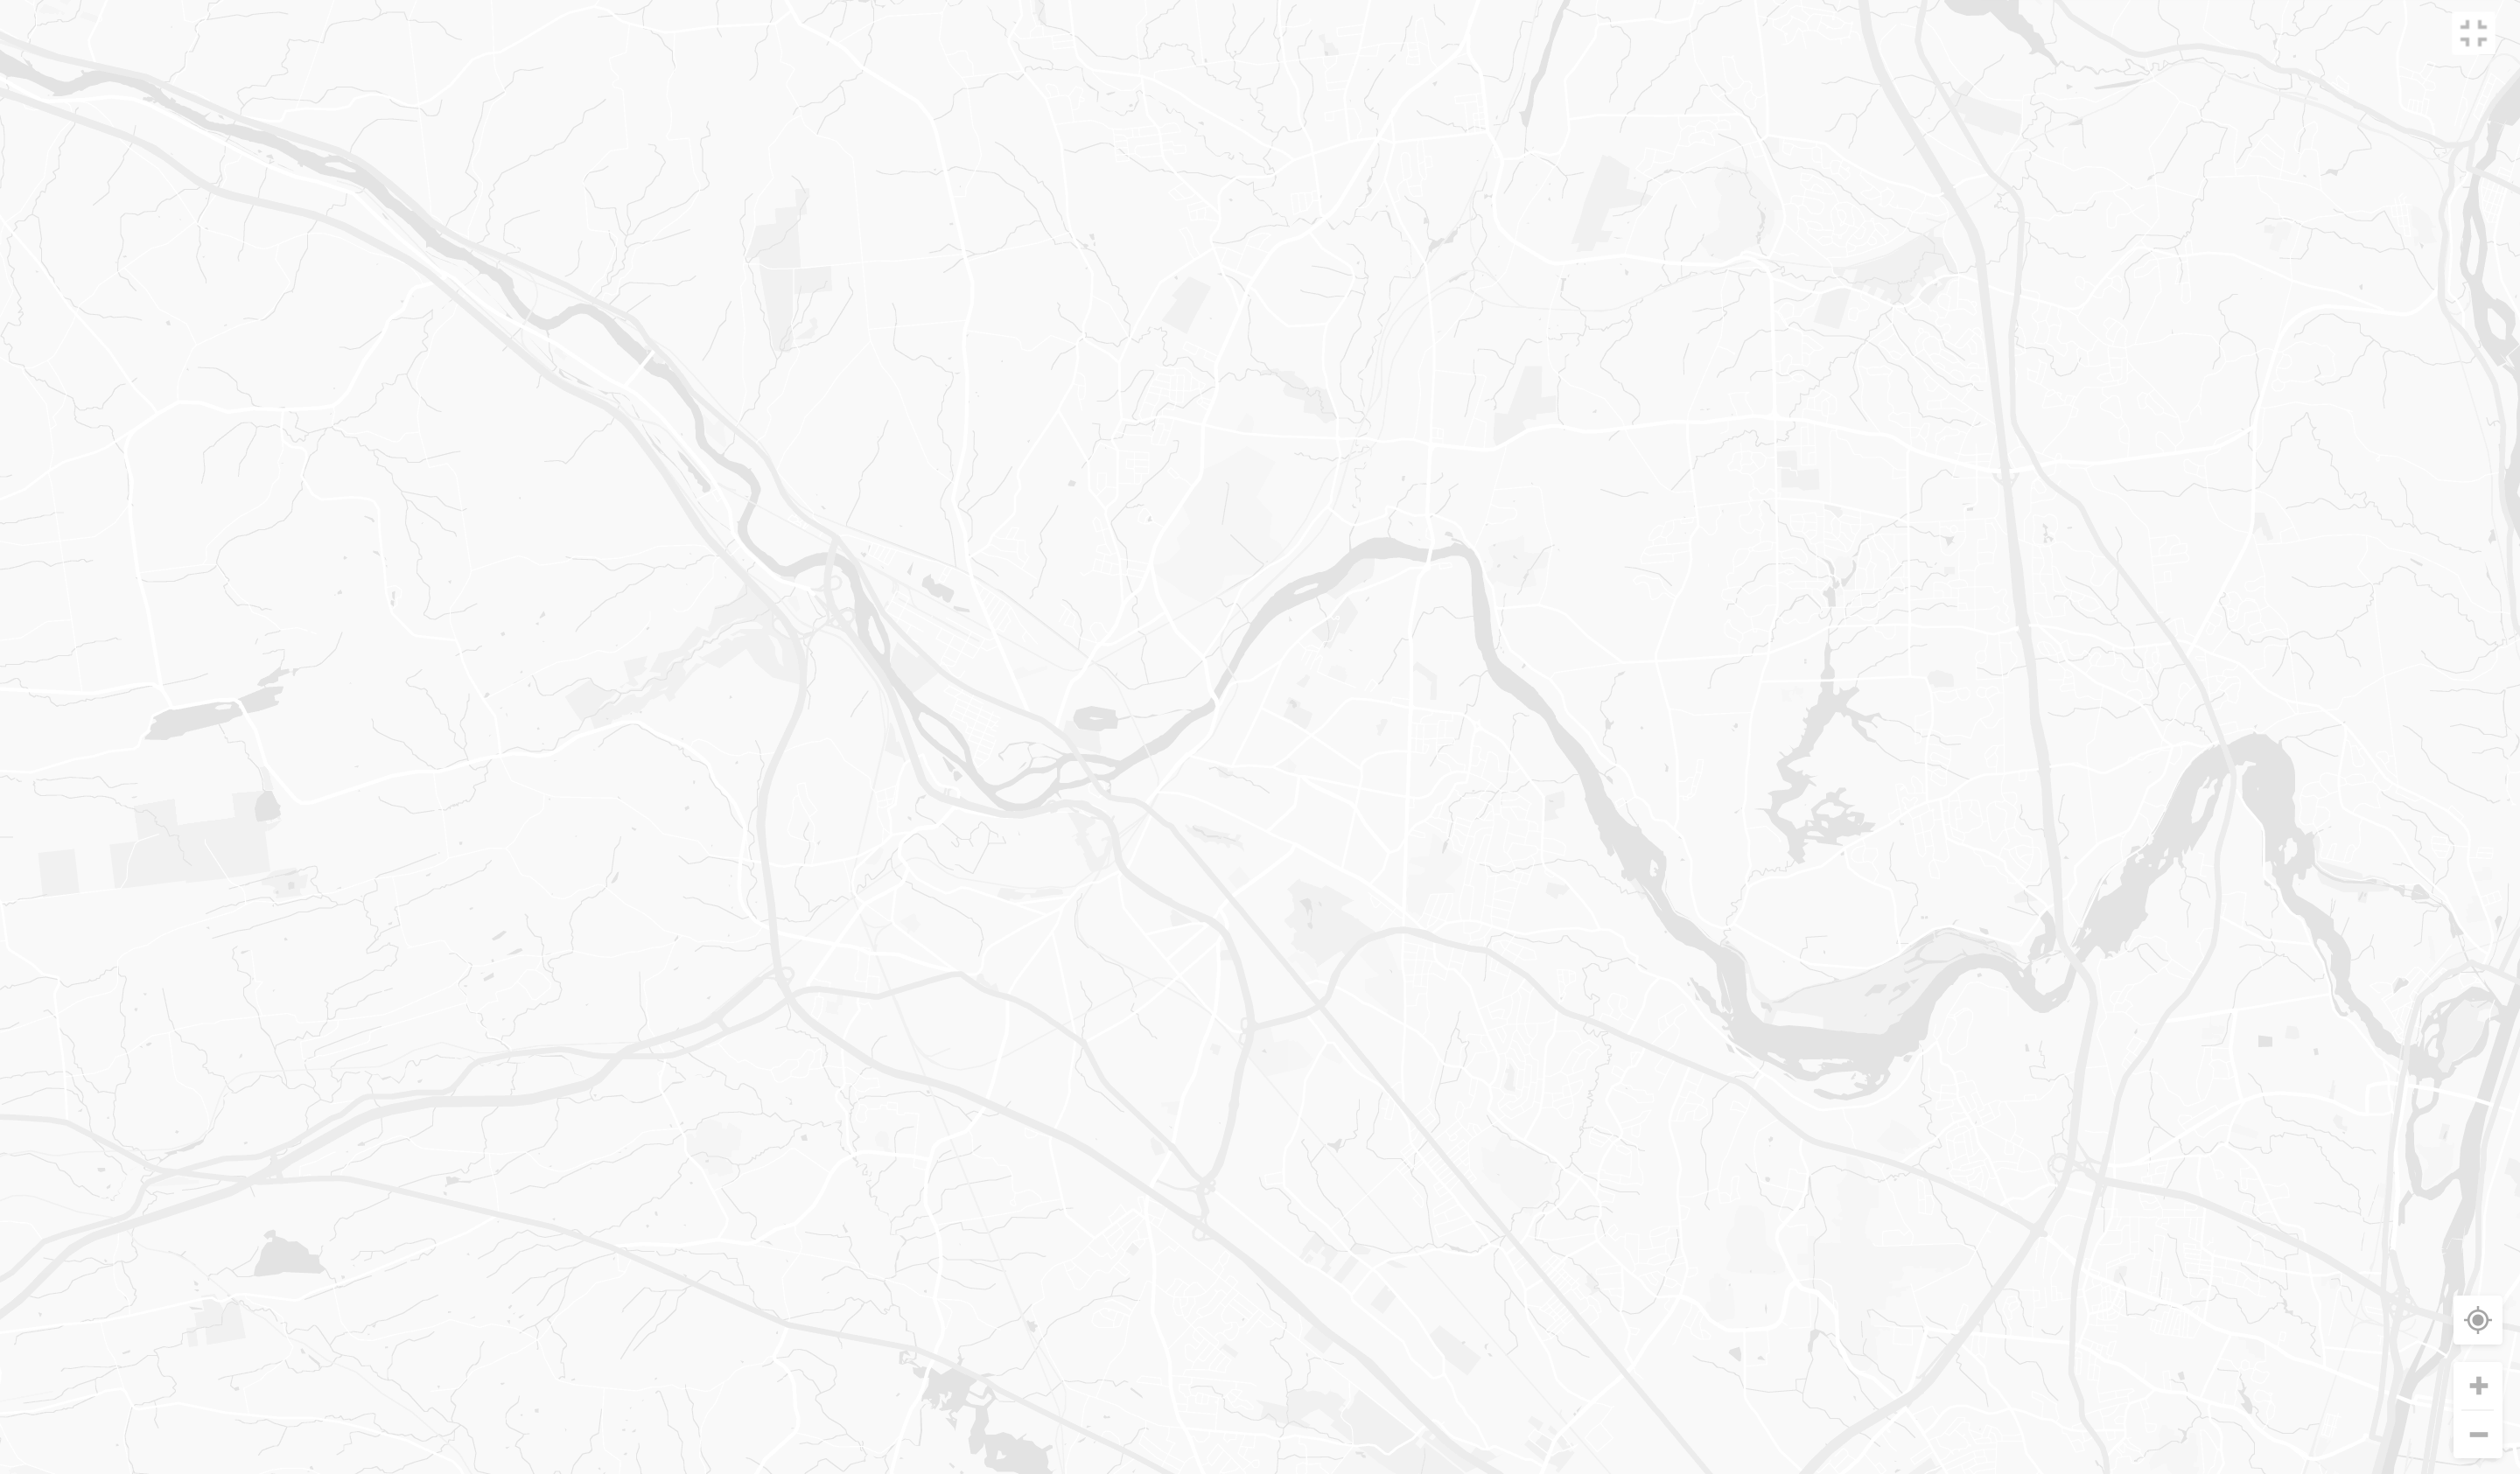
\includegraphics[height=\paperheight]{figs/schenectady3}
%} 
\begin{frame}
  \titlepage
\end{frame}

% Uncomment these lines for an automatically generated outline.
%\begin{frame}{Outline}
%  \tableofcontents
%\end{frame}

%\section{Introduction}
%
%\begin{frame}{Introduction}
%
%\begin{itemize}
%  \item Your introduction goes here!
%  \item Use \texttt{itemize} to organize your main points.
%\end{itemize}
%
%\vskip 1cm
%
%\begin{block}{Examples}
%Some examples of commonly used commands and features are included, to help you get started.
%\end{block}
%
%\end{frame}
%
%\section{Some \LaTeX{} Examples}
%
%\subsection{Tables and Figures}
%
%\begin{frame}{Tables and Figures}
%
%\begin{itemize}
%\item Use \texttt{tabular} for basic tables --- see Table~\ref{tab:widgets}, for example.
%\item You can upload a figure (JPEG, PNG or PDF) using the files menu. 
%\item To include it in your document, use the \texttt{includegraphics} command (see the comment below in the source code).
%\end{itemize}
%
%% Commands to include a figure:
%%\begin{figure}
%%\includegraphics[width=\textwidth]{your-figure's-file-name}
%%\caption{\label{fig:your-figure}Caption goes here.}
%%\end{figure}
%
%\begin{table}
%\centering
%\begin{tabular}{l|r}
%Item & Quantity \\\hline
%Widgets & 42 \\
%Gadgets & 13
%\end{tabular}
%\caption{\label{tab:widgets}An example table.}
%\end{table}
%
%\end{frame}
%
%\subsection{Mathematics}
%
%\begin{frame}{Readable Mathematics}
%
%Let $X_1, X_2, \ldots, X_n$ be a sequence of independent and identically distributed random variables with $\text{E}[X_i] = \mu$ and $\text{Var}[X_i] = \sigma^2 < \infty$, and let
%$$S_n = \frac{X_1 + X_2 + \cdots + X_n}{n}
%      = \frac{1}{n}\sum_{i}^{n} X_i$$
%denote their mean. Then as $n$ approaches infinity, the random variables $\sqrt{n}(S_n - \mu)$ converge in distribution to a normal $\mathcal{N}(0, \sigma^2)$.
%
%\end{frame}

\section{Introduction}

\begin{frame}{Introduction}

\begin{columns}
\column{0.5\textwidth}
    \begin{itemize}
        \item Routing for recreational cyclists is different than traditional routing problems.
        \item Cyclists prefer longer more scenic routes, not the shortest one. 
        \item Our focus is on \emph{circular} routes.   
    \end{itemize}
\column{0.5\textwidth}
\begin{center}
\begin{figure}
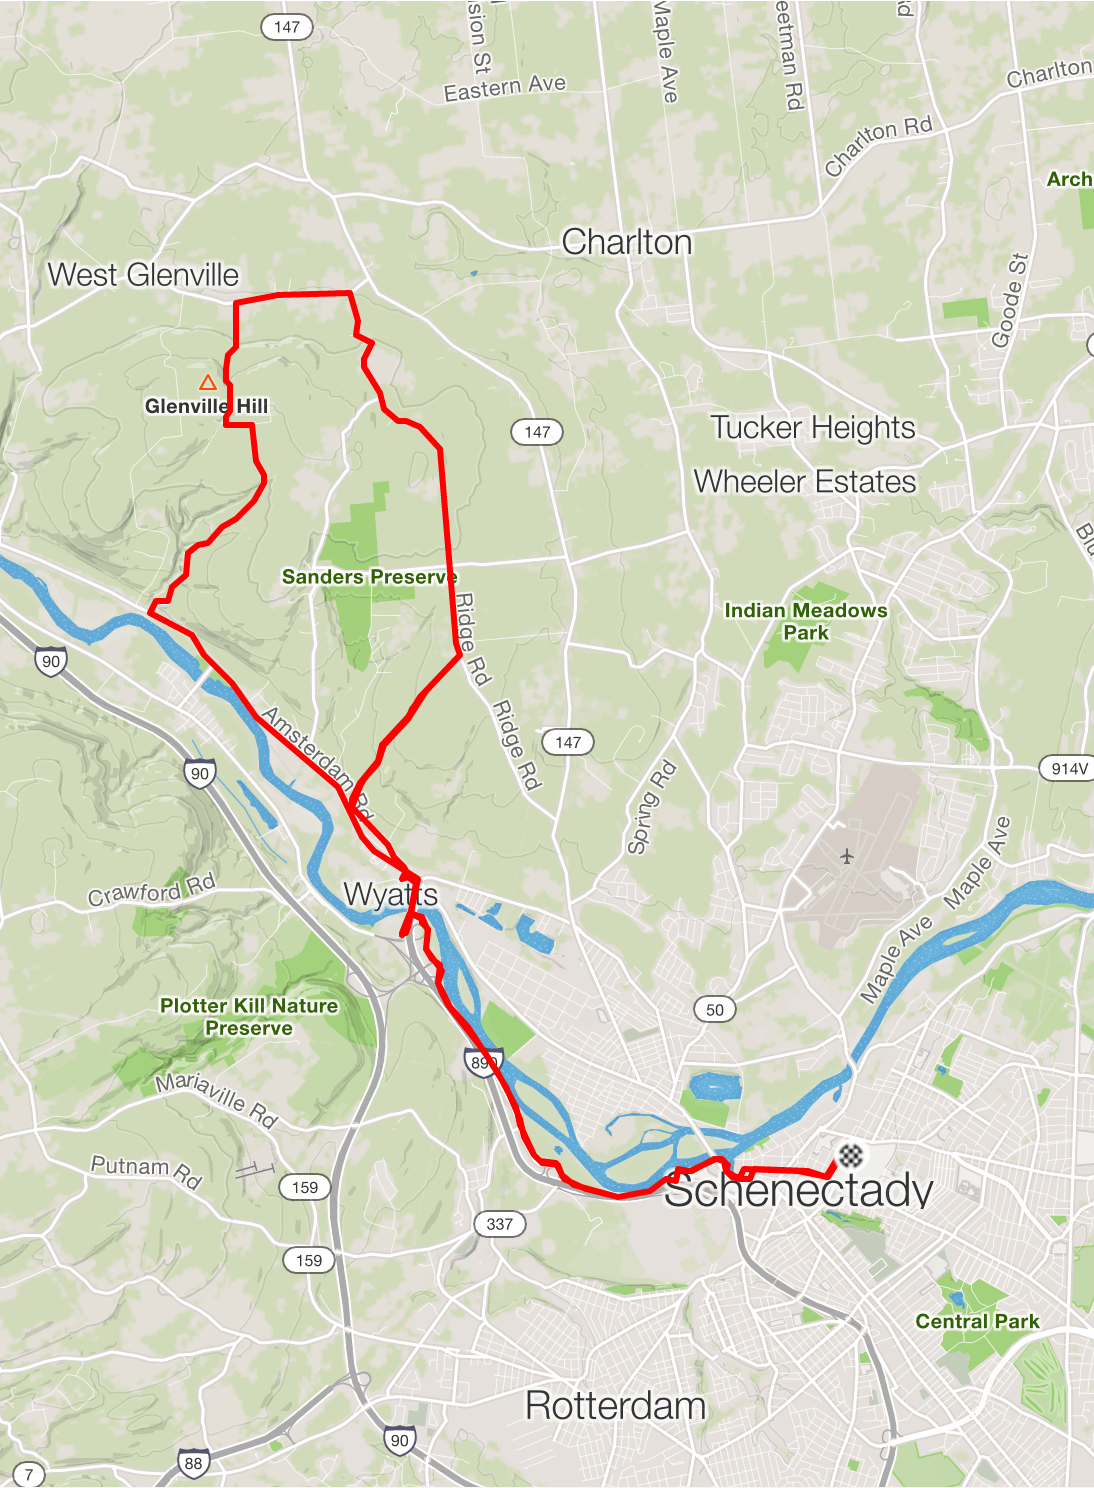
\includegraphics[width=0.98\textwidth]{figs/circular_route}
\caption{Circular bike route}
\end{figure}
\end{center}

\end{columns}


\end{frame}


\begin{frame}{Informal Problem Statement}
    Given:
    \begin{itemize}
        \item A road network
        \item A starting location
        \item A distance budget
    \end{itemize}
    \vspace{0.3cm}
    \emph{Goal:} Find the ``best" bike route which starts and ends at the specified location and is no longer than the budget.
\end{frame}

\begin{frame}{Related Work}
Previous literature models this problem as an instance of the\\\textbf{Arc Orienteering Problem (AOP)}.
\begin{figure}
    \tikzsetnextfilename{aop_1}
    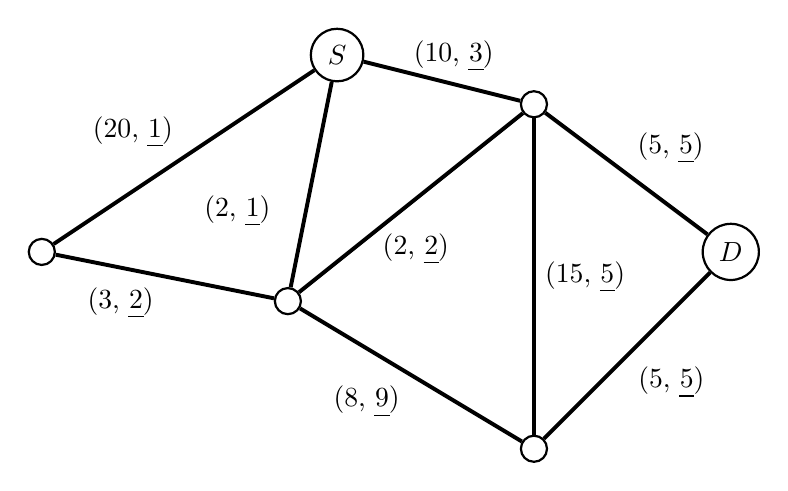
\begin{tikzpicture}[auto,x=1.25cm, y=1.25cm,line width=0.5mm]
        
        \begin{scope}[every node/.style={circle,thick,draw}]
        \node(1) at (0,0) {$S$};
        \node(2) at (2, -0.5) {};
        \node(3) at (4, -2) {$D$};
        \node(4) at (2, -4) {};
        \node(5) at (-0.5, -2.5) {};
        \node(6) at (-3, -2) {};
        \end{scope}
        
        \draw (1) -- node[xshift=-0.5cm] {(10, \ul{3})} (2);
        \draw (2) -- node {(5, \ul{5})} (3);
        \draw (3) -- node {(5, \ul{5})} (4);
        \draw (2) -- node {(15, \ul{5})} (4);
        \draw (2) -- node[yshift=-0.25cm, xshift=-0.5cm] {(2, \ul{2})}(5);
        \draw (4) -- node {(8, \ul{9})}(5);
        \draw (5) -- node {(3, \ul{2})} (6);
        \draw (6) -- node[] {(20, \ul{1})} (1);
        \draw (1) -- node [xshift=-1.5cm]{(2, \ul{1})} (5);
    \end{tikzpicture}
    \caption{AOP Instance - Edge label: ($score$, \ul{$cost$}) Budget: 10}
    \end{figure}  
\end{frame}

\begin{frame}{Arc Orienteering Example}
\begin{figure}
        \tikzsetnextfilename{aop_2}
        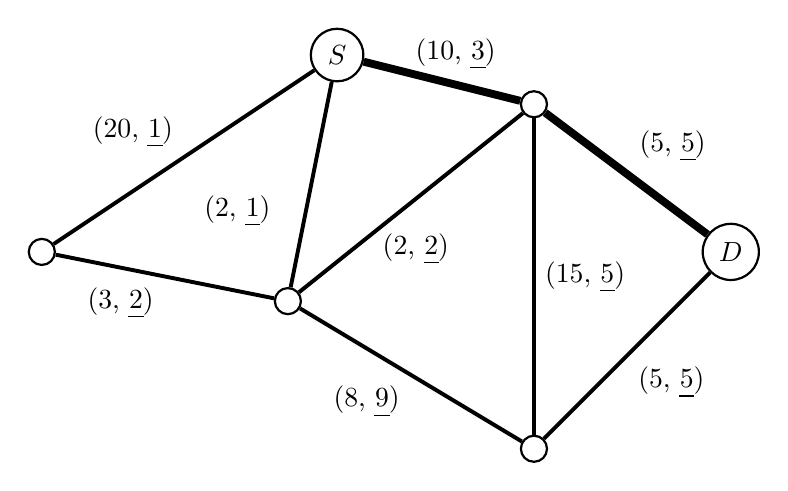
\begin{tikzpicture}[auto,x=1.25cm, y=1.25cm,line width=0.5mm]
    
        \begin{scope}[every node/.style={circle,thick,draw}]
        \node(1) at (0,0) {$S$};
        \node(2) at (2, -0.5) {};
        \node(3) at (4, -2) {$D$};
        \node(4) at (2, -4) {};
        \node(5) at (-0.5, -2.5) {};
        \node(6) at (-3, -2) {};
        \end{scope}
        
        \draw (1)[line width=1mm] -- node[xshift=-0.5cm] {(10, \ul{3})} (2);
        \draw[line width=1mm]  (2) -- node {(5, \ul{5})} (3);
        \draw (3) -- node {(5, \ul{5})} (4);
        \draw (2) -- node {(15, \ul{5})} (4);
        \draw (2) -- node[yshift=-0.25cm, xshift=-0.5cm] {(2, \ul{2})}(5);
        \draw (4) -- node {(8, \ul{9})}(5);
        \draw (5) -- node {(3, \ul{2})} (6);
        \draw (6) -- node[] {(20, \ul{1})} (1);
        \draw (1) -- node [xshift=-1.5cm]{(2, \ul{1})} (5);
    \end{tikzpicture}
    \caption{Shortest Path: ($score = 15$, \ul{$cost = 8$}) Budget: 10}
    \end{figure}
\end{frame}


\begin{frame}{Arc Orienteering Example}
\begin{figure}
        \tikzsetnextfilename{aop_3}
        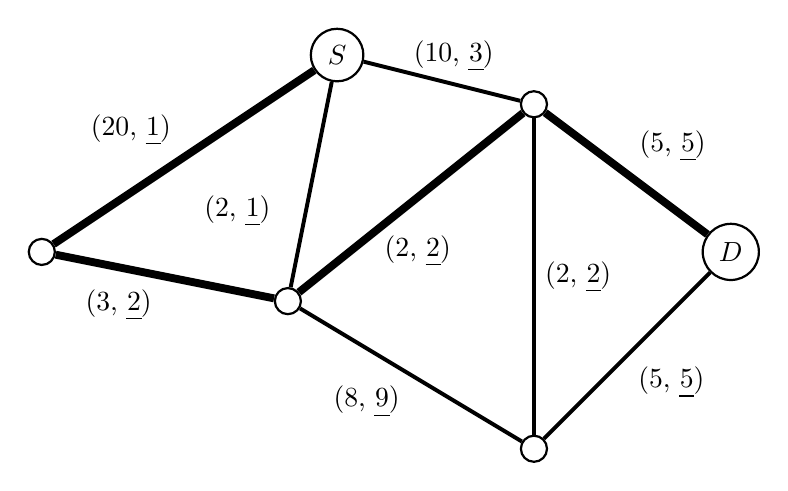
\begin{tikzpicture}[auto,x=1.25cm, y=1.25cm,line width=0.5mm]
    
        \begin{scope}[every node/.style={circle,thick,draw}]
        \node(1) at (0,0) {$S$};
        \node(2) at (2, -0.5) {};
        \node(3) at (4, -2) {$D$};
        \node(4) at (2, -4) {};
        \node(5) at (-0.5, -2.5) {};
        \node(6) at (-3, -2) {};
        \end{scope}
        
        \draw (1) -- node[xshift=-0.5cm] {(10, \ul{3})} (2);
        \draw[line width=1mm]  (2) -- node {(5, \ul{5})} (3);
        \draw (3) -- node {(5, \ul{5})} (4);
        \draw (2) -- node {(2, \ul{2})} (4);
        \draw[line width=1mm] (2) -- node[yshift=-0.25cm, xshift=-0.5cm] {(2, \ul{2})}(5);
        \draw (4) -- node {(8, \ul{9})}(5);
        \draw[line width=1mm] (5) -- node {(3, \ul{2})} (6);
        \draw[line width=1mm] (6) -- node[] {(20, \ul{1})} (1);
        \draw (1) -- node [xshift=-1.5cm]{(2, \ul{1})} (5);
    \end{tikzpicture}
    \caption{Optimal Path: ($score = 30$, \ul{$cost = 10$}) Budget: 10}
    \end{figure}

\end{frame}

\section{Problem Statement}
\begin{frame}{Revised Problem Statement}
Given:
\begin{itemize}
    \item A graph where each arc has the following:
    \begin{itemize}
        \item A cost (e.g., distance)
        \item A score (e.g., number denoting the bike safety of the road)
    \end{itemize}
    \item A starting and ending node
    \item A distance budget
\end{itemize}
\emph{Goal:} Produce a \emph{path} with specified start and end which visits some subset of the graph nodes maximizing score and is within the distance budget.
\end{frame}

\section{Methods}
\begin{frame}{Methods}
    The AOP is NP-Hard:
    \begin{itemize}
        \item Our focus is on heuristic algorithms for the AOP.
        \item \textbf{Iterated Local Search (ILS)} is the algorithm of interest.
    \end{itemize}
    
    \begin{alertblock}{Research Question:}
        To what extent can ILS algorithms be improved to generate better bike routes?
    \end{alertblock}
    \vspace{0.3cm}
    We implemented two ILS algorithms using:
    \begin{itemize}
        \item \textbf{GraphHopper}: An open source routing library.
        \item \textbf{OpenStreetMap}: An open mapping dataset.
    \end{itemize}
    

\end{frame}

\begin{frame}{Methods: GraphHopper Routing Engine}
\begin{figure}
    \makebox[\linewidth]{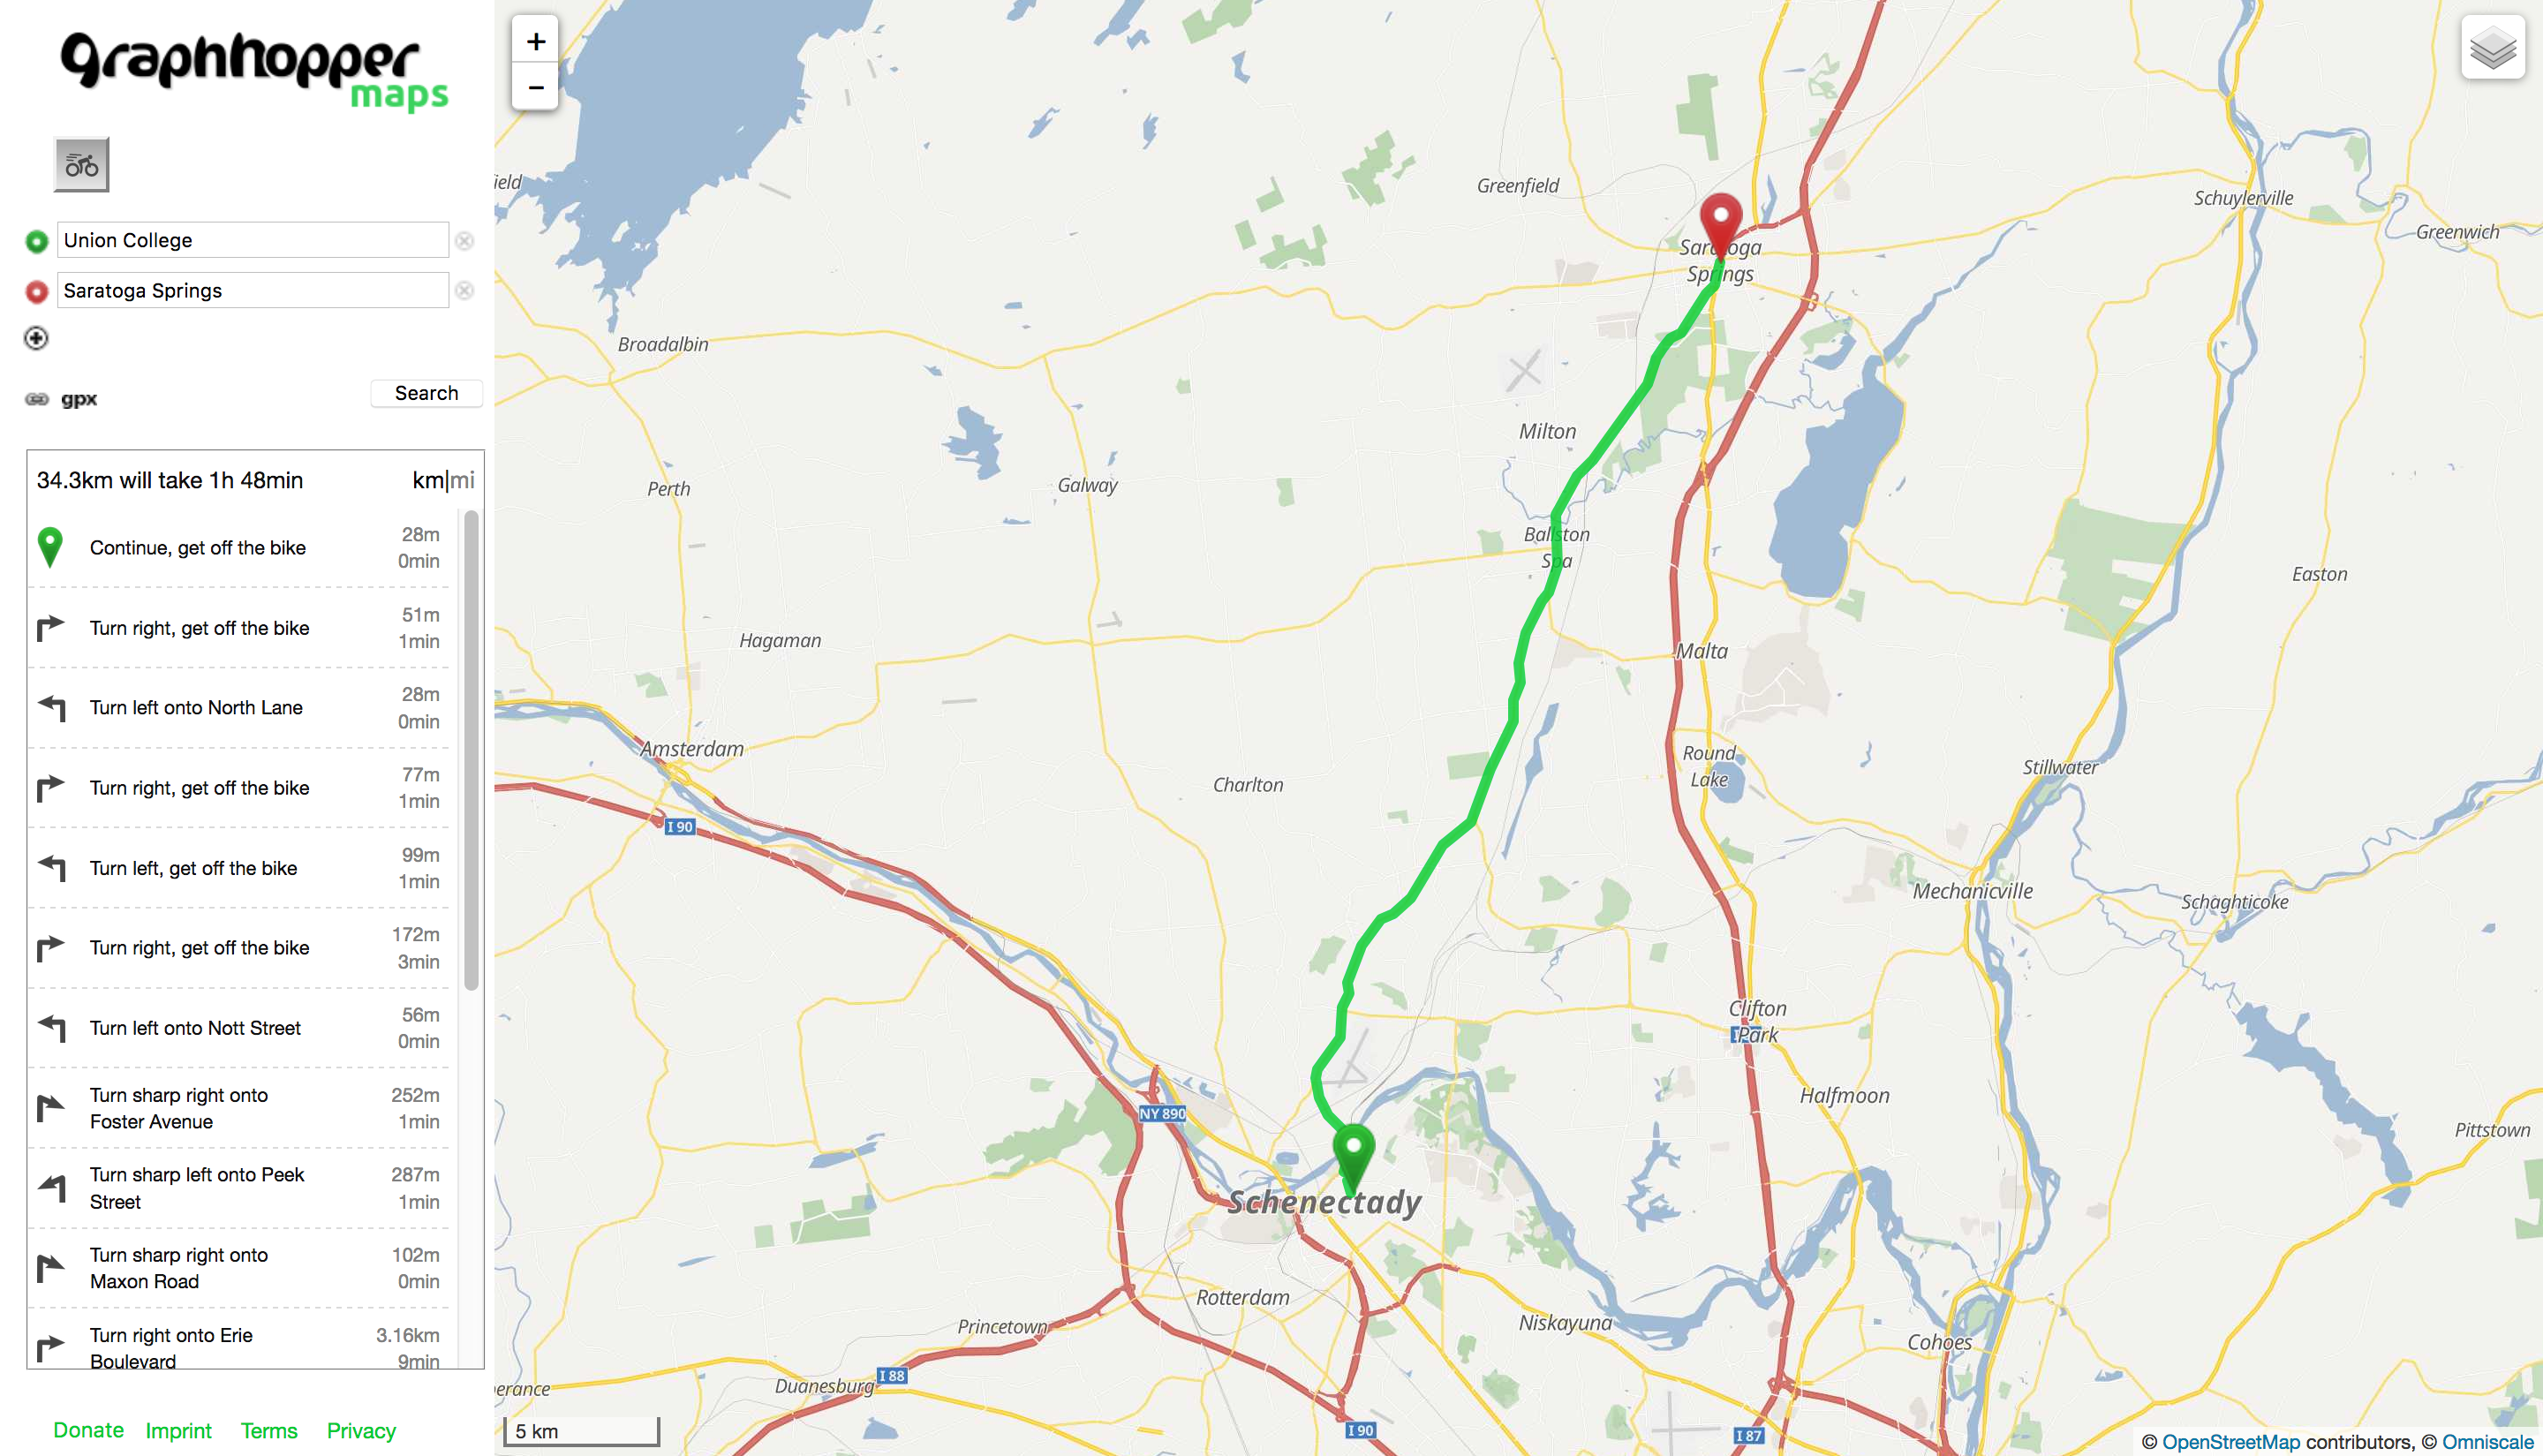
\includegraphics[width=\paperwidth]{figs/graphhopper}}
\caption{Shortest path Union $\rightarrow$ Saratoga Springs}
\end{figure}
\end{frame}



\begin{frame}{DFS Algorithm \cite{verbeeck2014extension}}
    \begin{itemize}
        \item Uses modified \textbf{Depth First Search} with max depth.
        \item Precomputes all-pairs shortest path for feasibility checking.
        \item Returns first path found fitting criteria. 
    \end{itemize}

\begin{figure}
\begin{center}
    \tikzsetnextfilename{arc_feasability}
 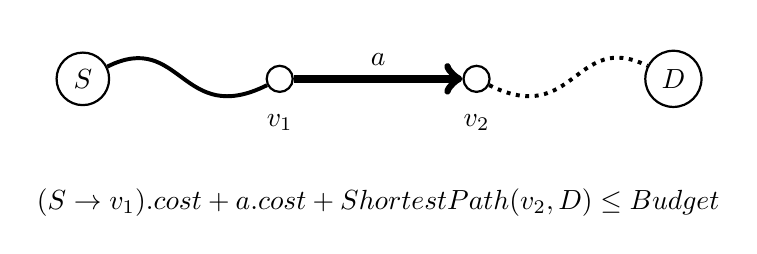
\begin{tikzpicture}[auto,x=1.25cm, y=1.25cm,line width=0.5mm]
    \begin{scope}[every node/.style={circle,thick,draw}]
        \node(1) at (0,0) {$S$};
        \node(2) at (6, 0) {$D$};
        \node[label=below:$v_1$](3) at (2,0) {};
        \node[label=below:$v_2$](4) at (4,0) {};
        \end{scope}
        \draw (1) .. controls (1, 0.5) and (1, -0.5) .. (3);
        \draw[->, line width=1mm] (3) -- node{$a$}(4);
        \draw[dotted] (4) .. controls (5, -0.5) and (5, 0.5) .. (2);
        \node[below] at (3,-1) {$(S \rightarrow v_1).cost + a.cost + ShortestPath(v_2, D) \leq Budget$};
    \end{tikzpicture}
\end{center}
\caption{Arc feasibility checking}
\end{figure}
\end{frame}

\begin{frame}{DFS Algorithm \cite{verbeeck2014extension}}
\begin{figure}
\makebox[\linewidth]{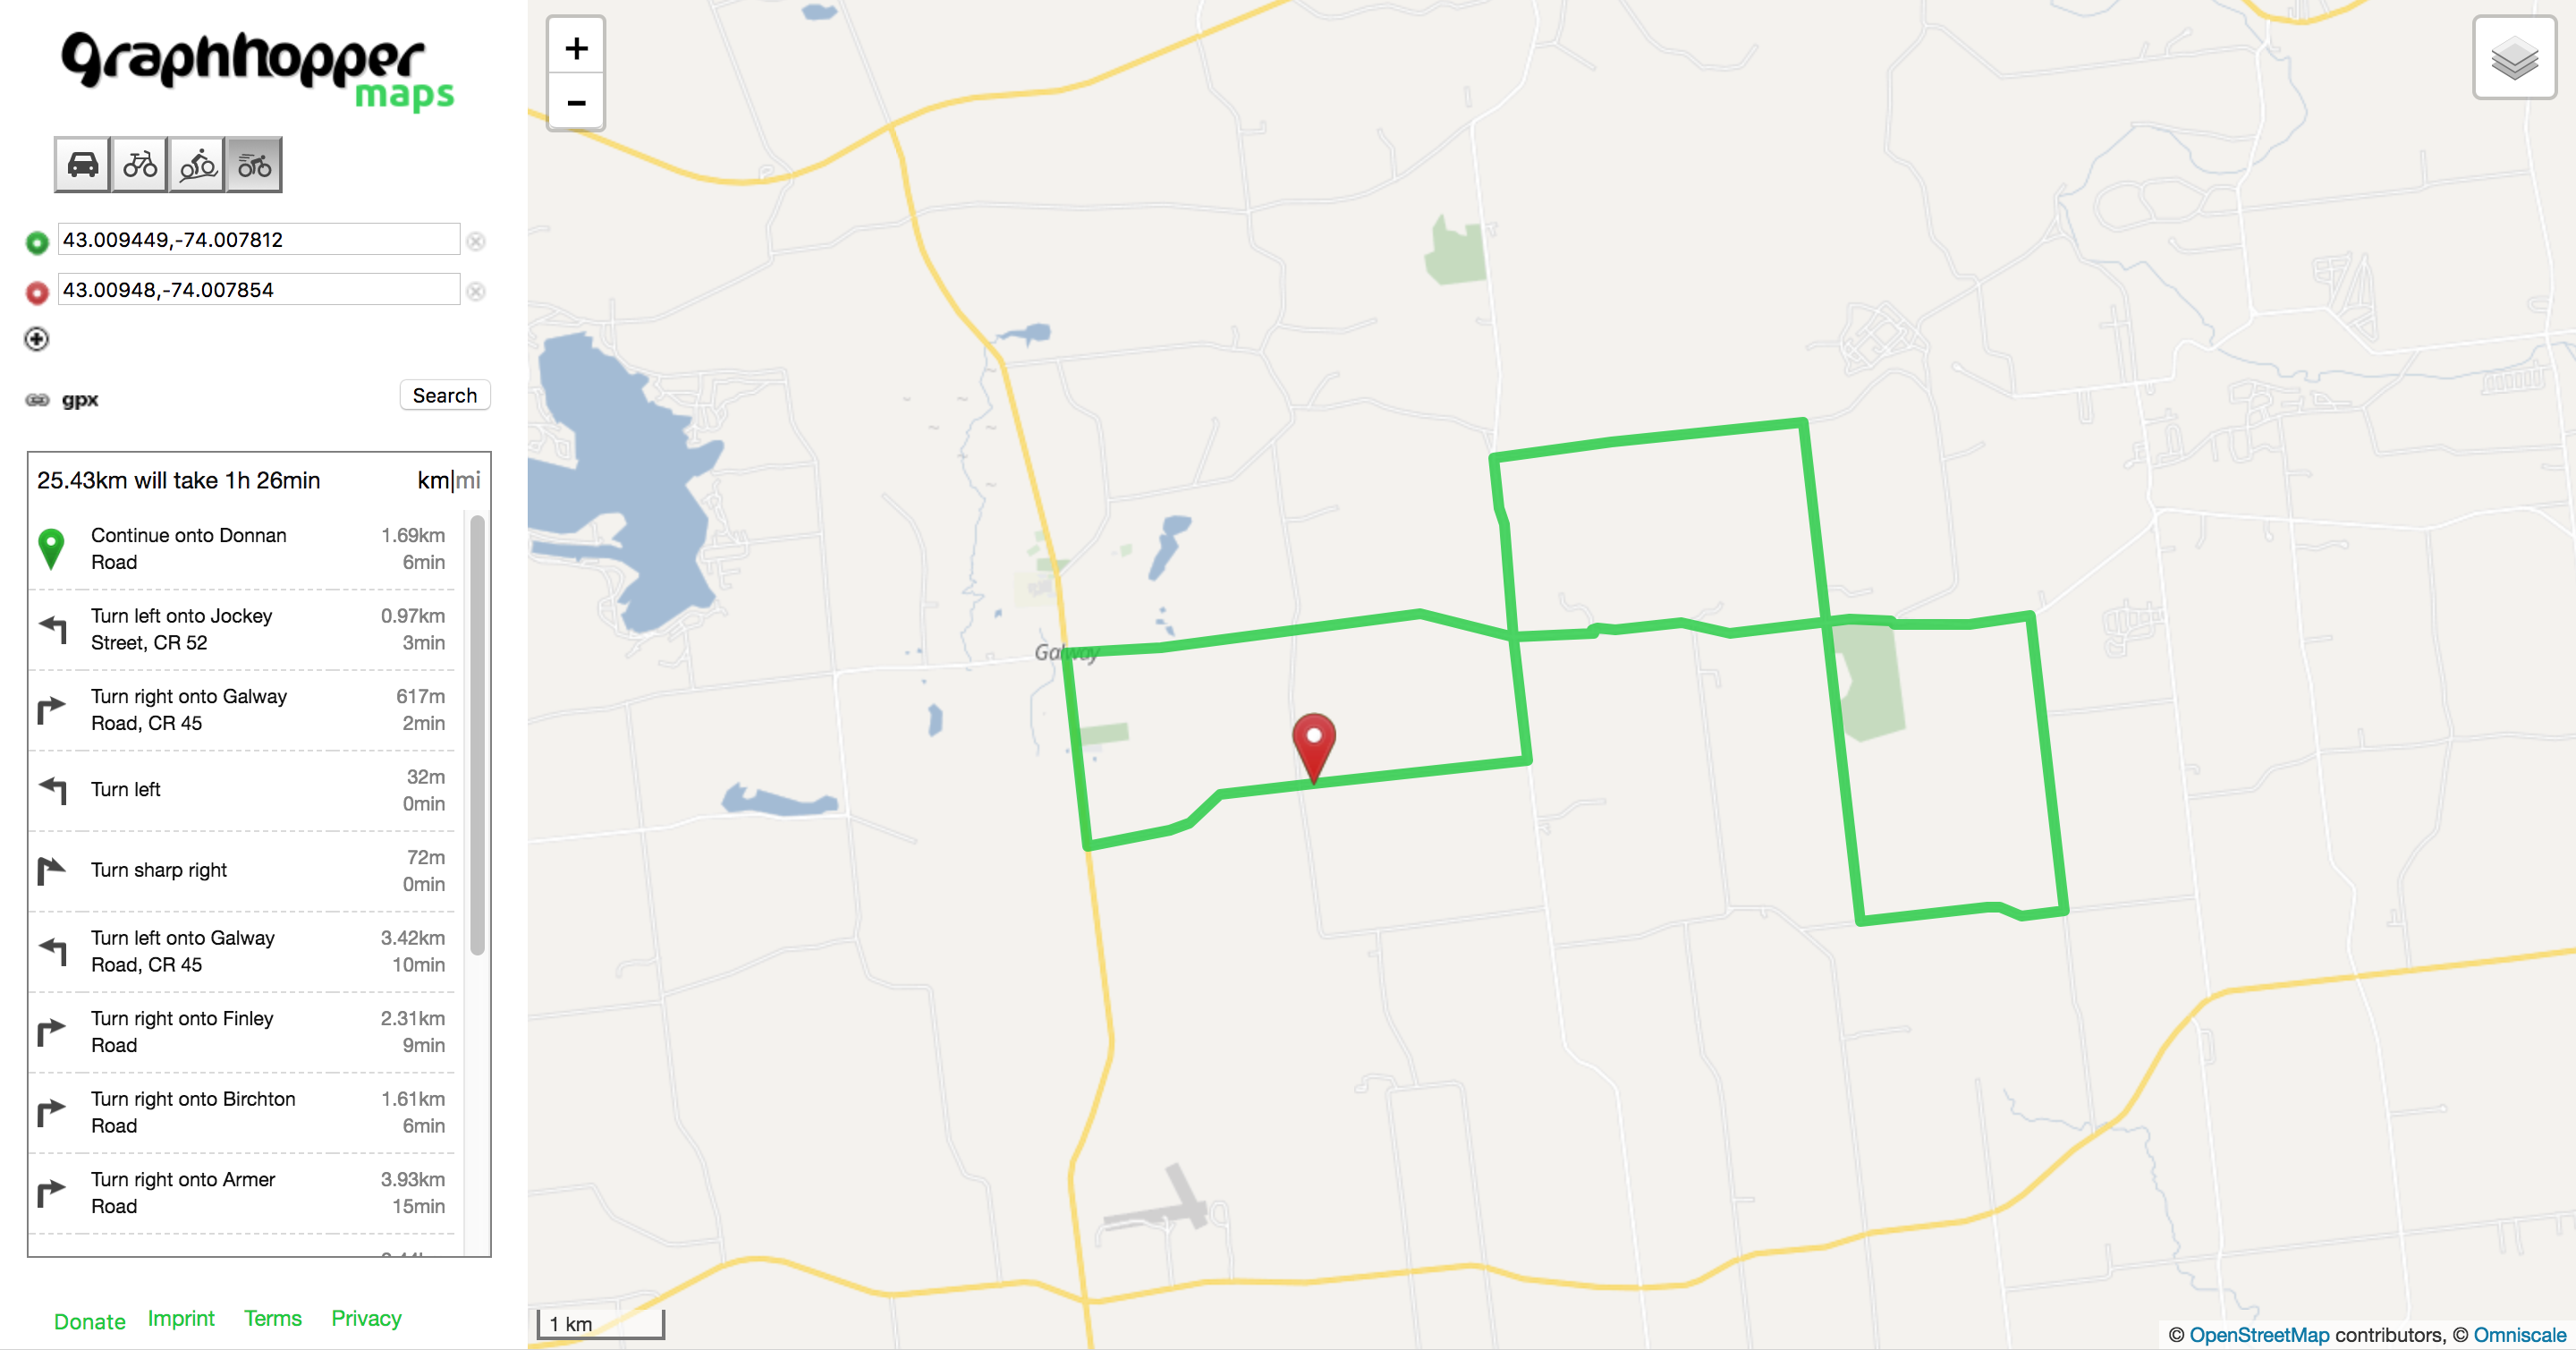
\includegraphics[width=\paperwidth]{figs/vva_route}}
\caption{DFS Algorithm Example Route}
\end{figure}
\end{frame}

\begin{frame}{DFS Algorithm \cite{verbeeck2014extension}}
Limitations:
\begin{itemize}
    \item Search space large in road dense areas.
    \item Requires pre-computed all-pairs shortest path.
    \item Does not penalize turns.
\end{itemize}
\begin{figure}
\begin{center}
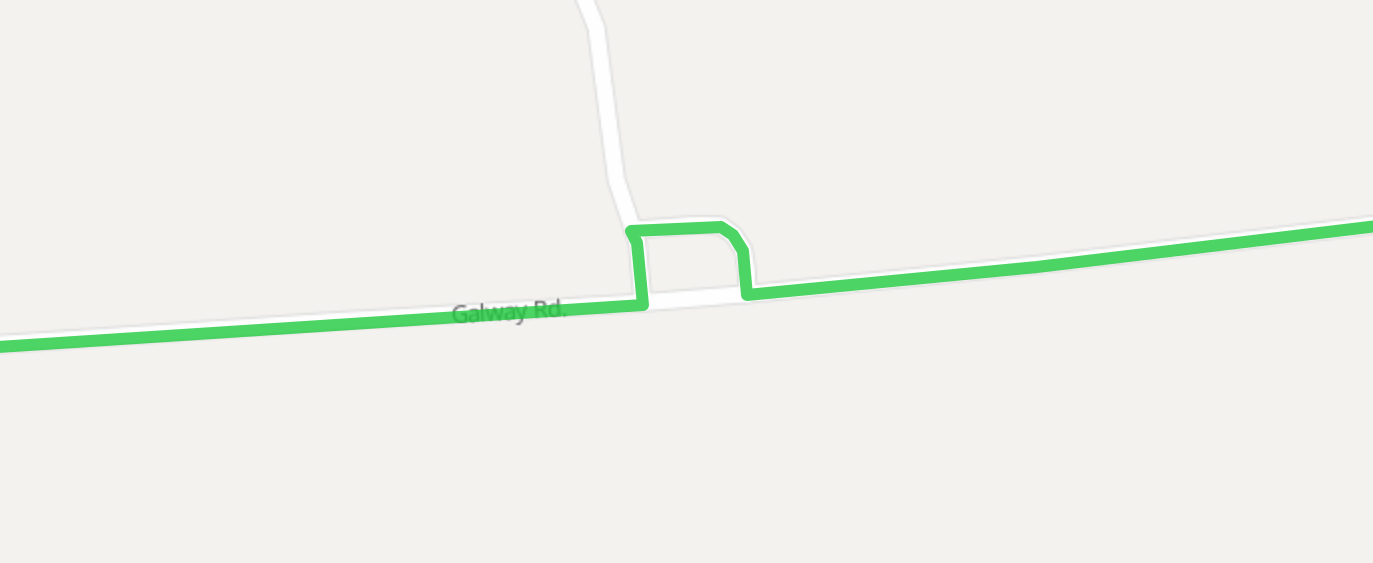
\includegraphics[width=0.8\textwidth]{figs/vva_route_turn}
\end{center}
\caption{Dangerous route turn}
\end{figure}
\end{frame}

\begin{frame}{Geometric Algorithm \cite{lu2015arc}}
\begin{itemize}
    \item Generates paths by ``gluing together" \textbf{Attractive Arcs} from a \textbf{Candidate Arc Set}.
    \item Uses spatial techniques to reduce search space.
    \item Uses online shortest path computations \cite{geisberger2008contraction}.
\end{itemize}

\begin{center}
\begin{figure}
\tikzsetnextfilename{ellipse_pruning}
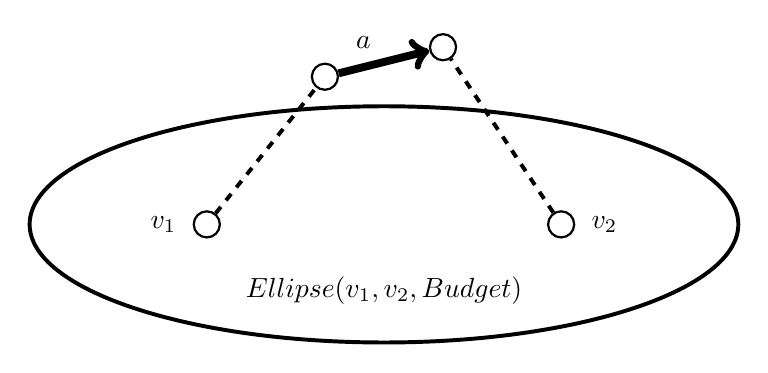
\begin{tikzpicture}[auto, x=1.5cm, y=0.75cm]
  \begin{scope}[every node/.style={circle,thick,draw}]
\node[label=left:$v_1$](1) at (0,0) {};
\node[label=right:$v_2$](2) at (3,0) {};
\node(4) at (1, 2.5) {};
\node(5) at (2, 3) {};
\end{scope}

\draw[dashed, line width=0.5mm] (1) -- (4);
\draw[dashed, line width=0.5mm] (2) -- (5);
\draw[->, line width=1mm] (4) -- node{$a$}(5);

\draw[line width=0.5mm] (1.5, 0) ellipse (4.5 cm and 1.5cm) node [below=15pt] {$Ellipse(v_1, v_2, Budget)$};
\end{tikzpicture}
\caption{Ellipse pruning technique}
\end{figure}
\end{center}
\end{frame}


\begin{frame}{Geometric Algorithm \cite{lu2015arc}}
\begin{figure}
\makebox[\linewidth]{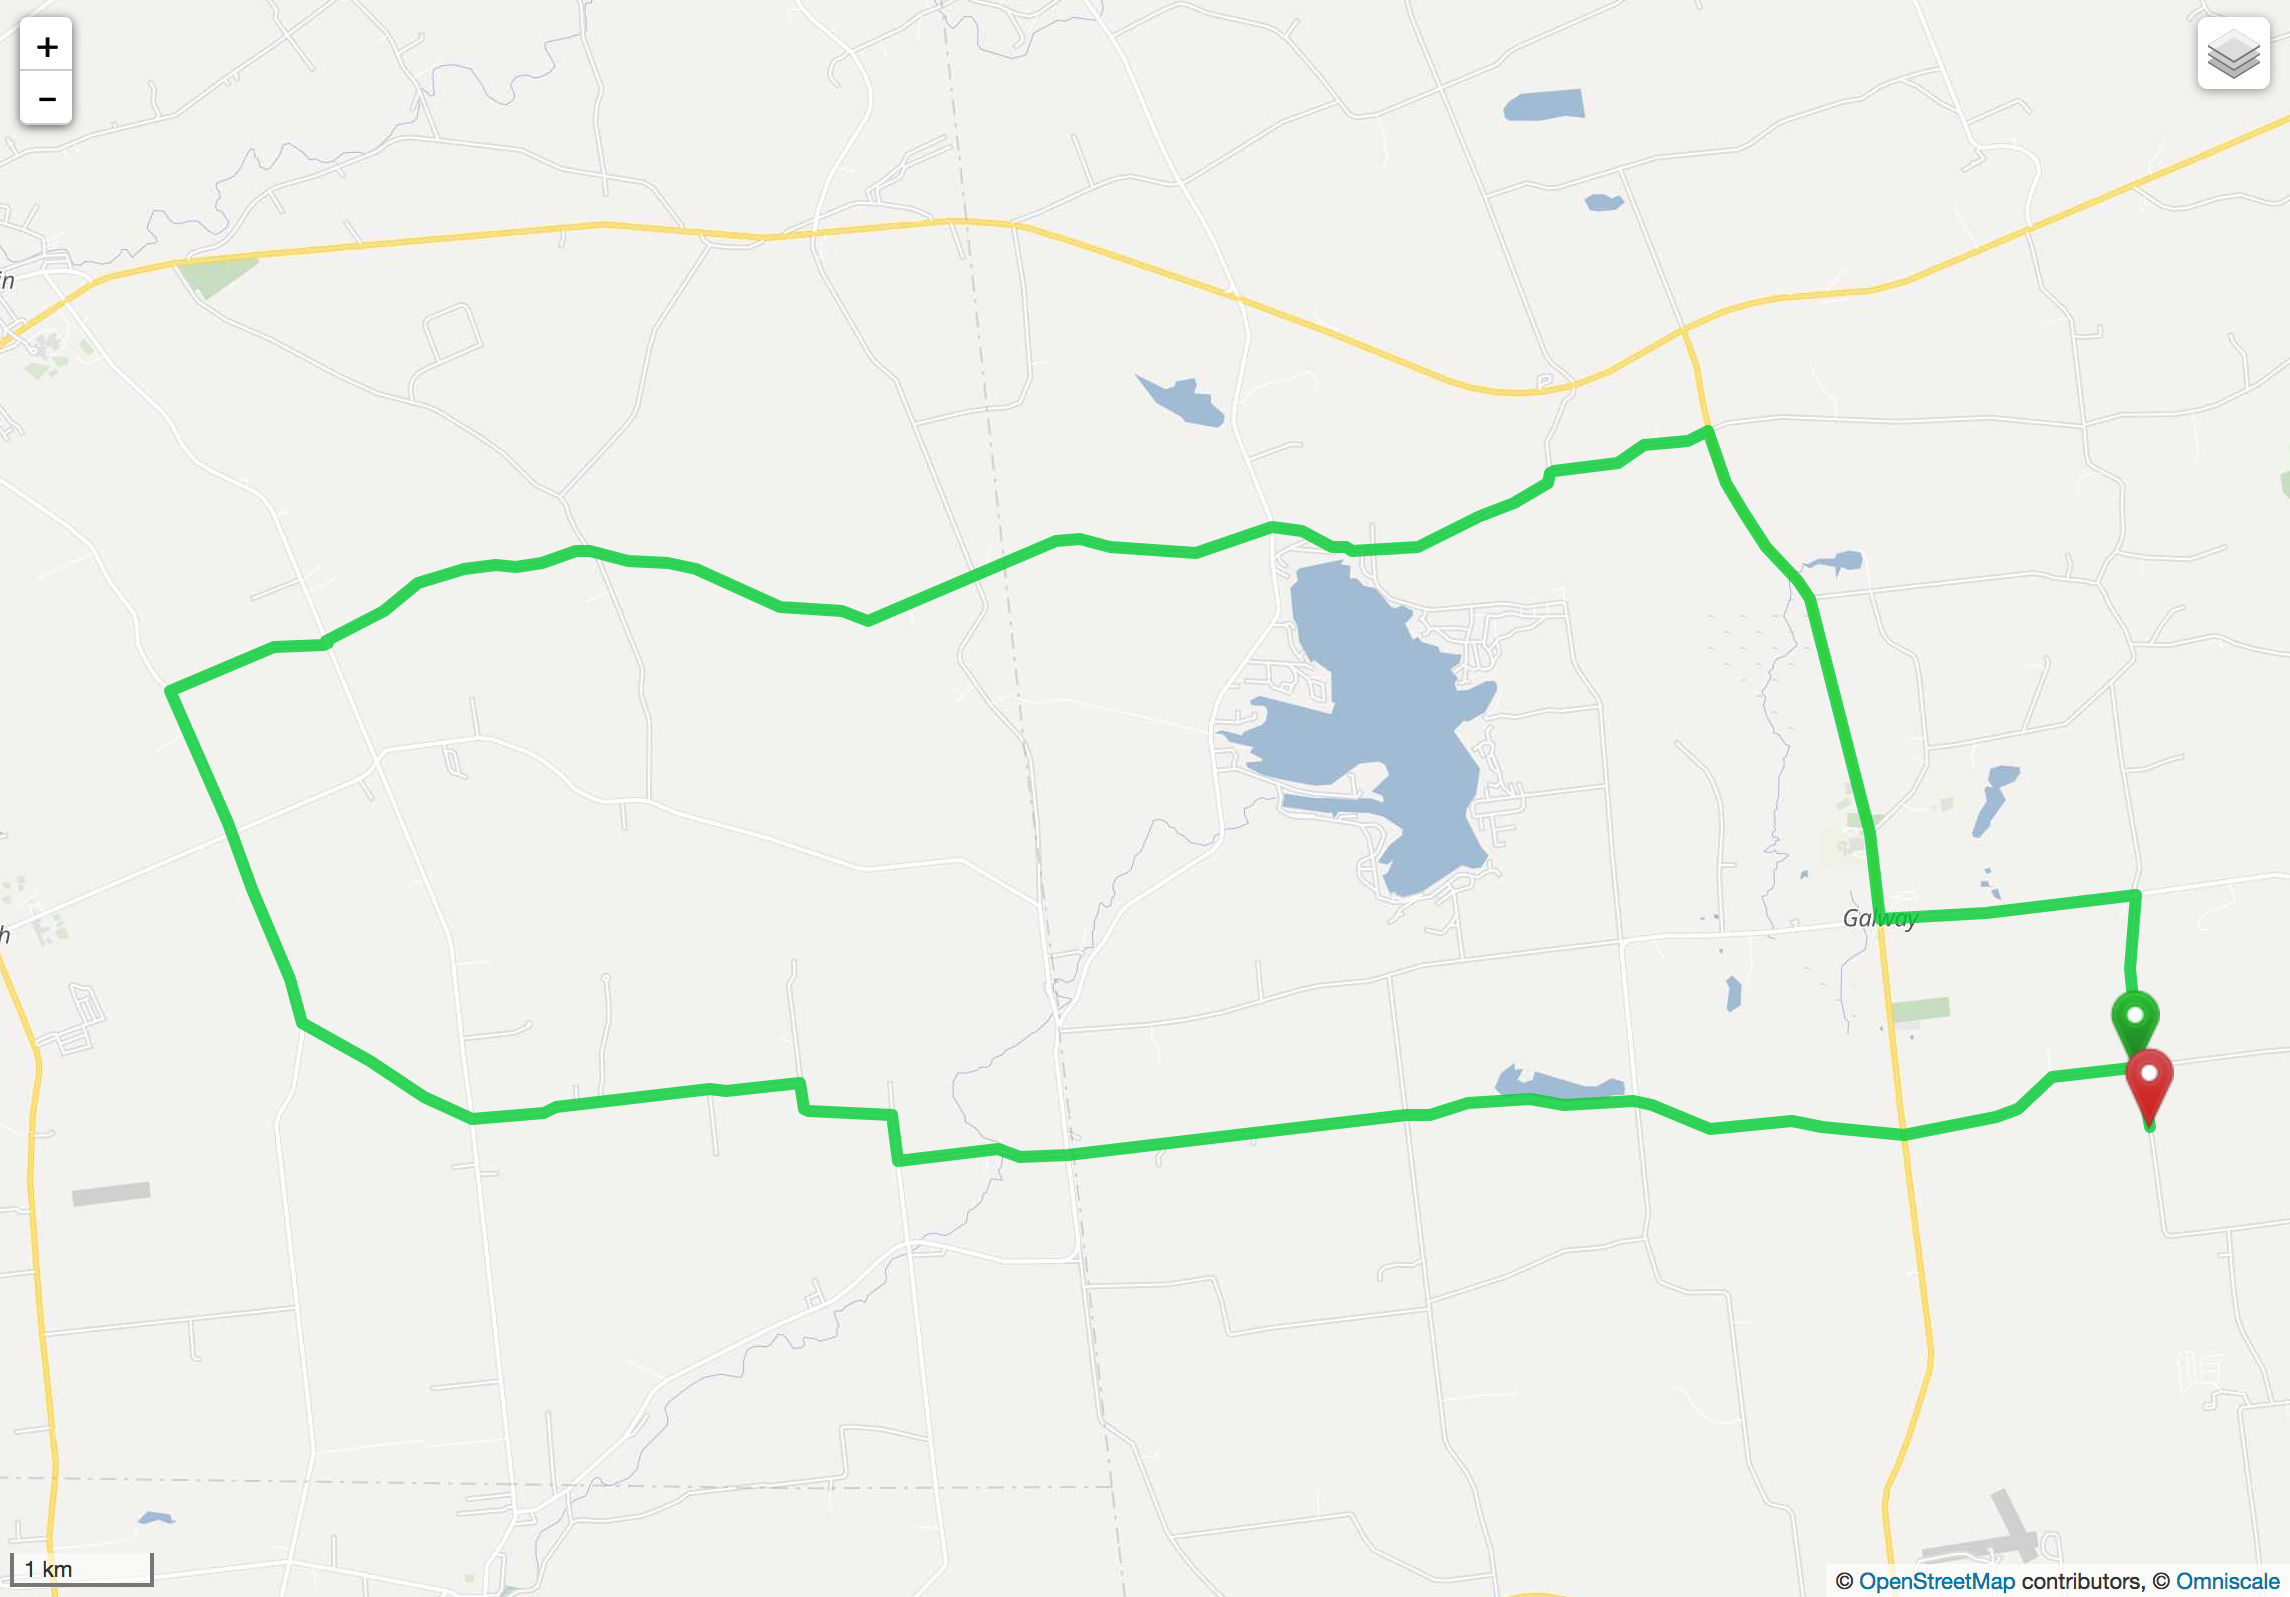
\includegraphics[width=\paperwidth]{figs/ls-route1}}
\caption{Perfectly circular route generated by Geometric Algorithm.}
\end{figure}
\end{frame}

\begin{frame}{Geometric Algorithm \cite{lu2015arc}}
\begin{figure}
\makebox[\linewidth]{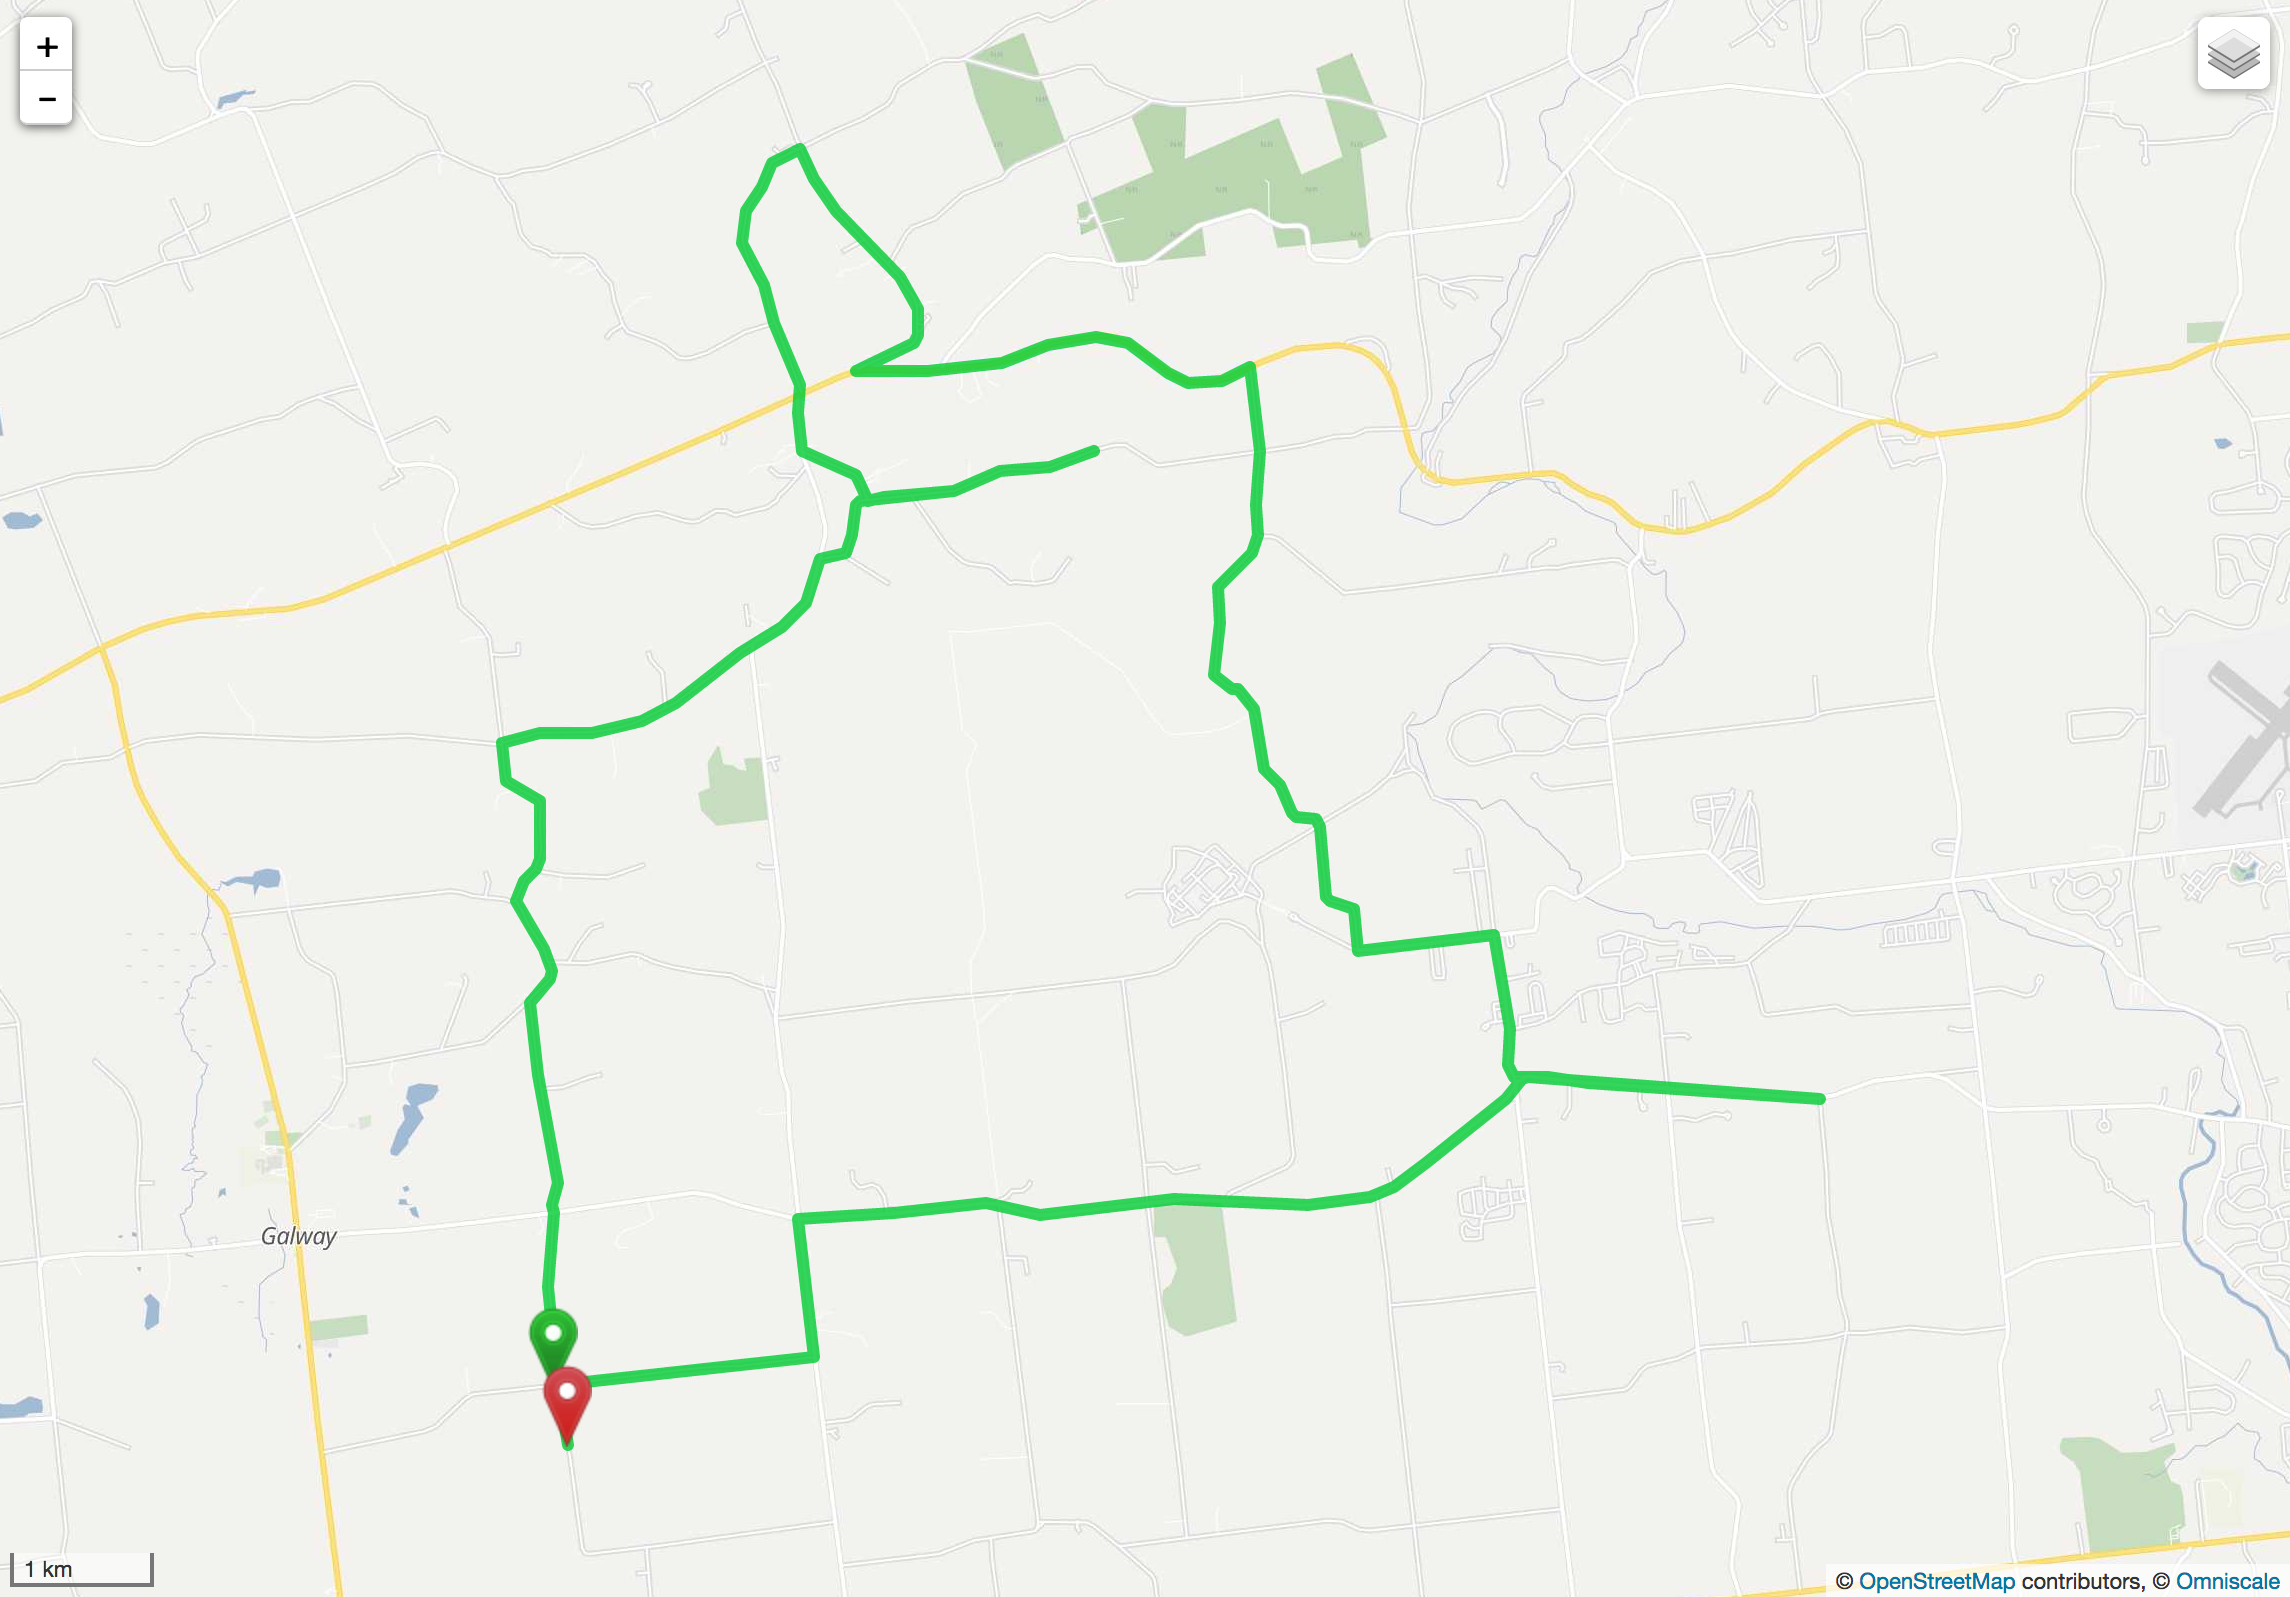
\includegraphics[width=\paperwidth]{figs/ls-route2}}
\caption{Route with backtracking generated by Geometric Algorithm.}
\end{figure}    
\end{frame}

\begin{frame}{Geometric Algorithm \cite{lu2015arc}}
\begin{figure}
\makebox[\linewidth]{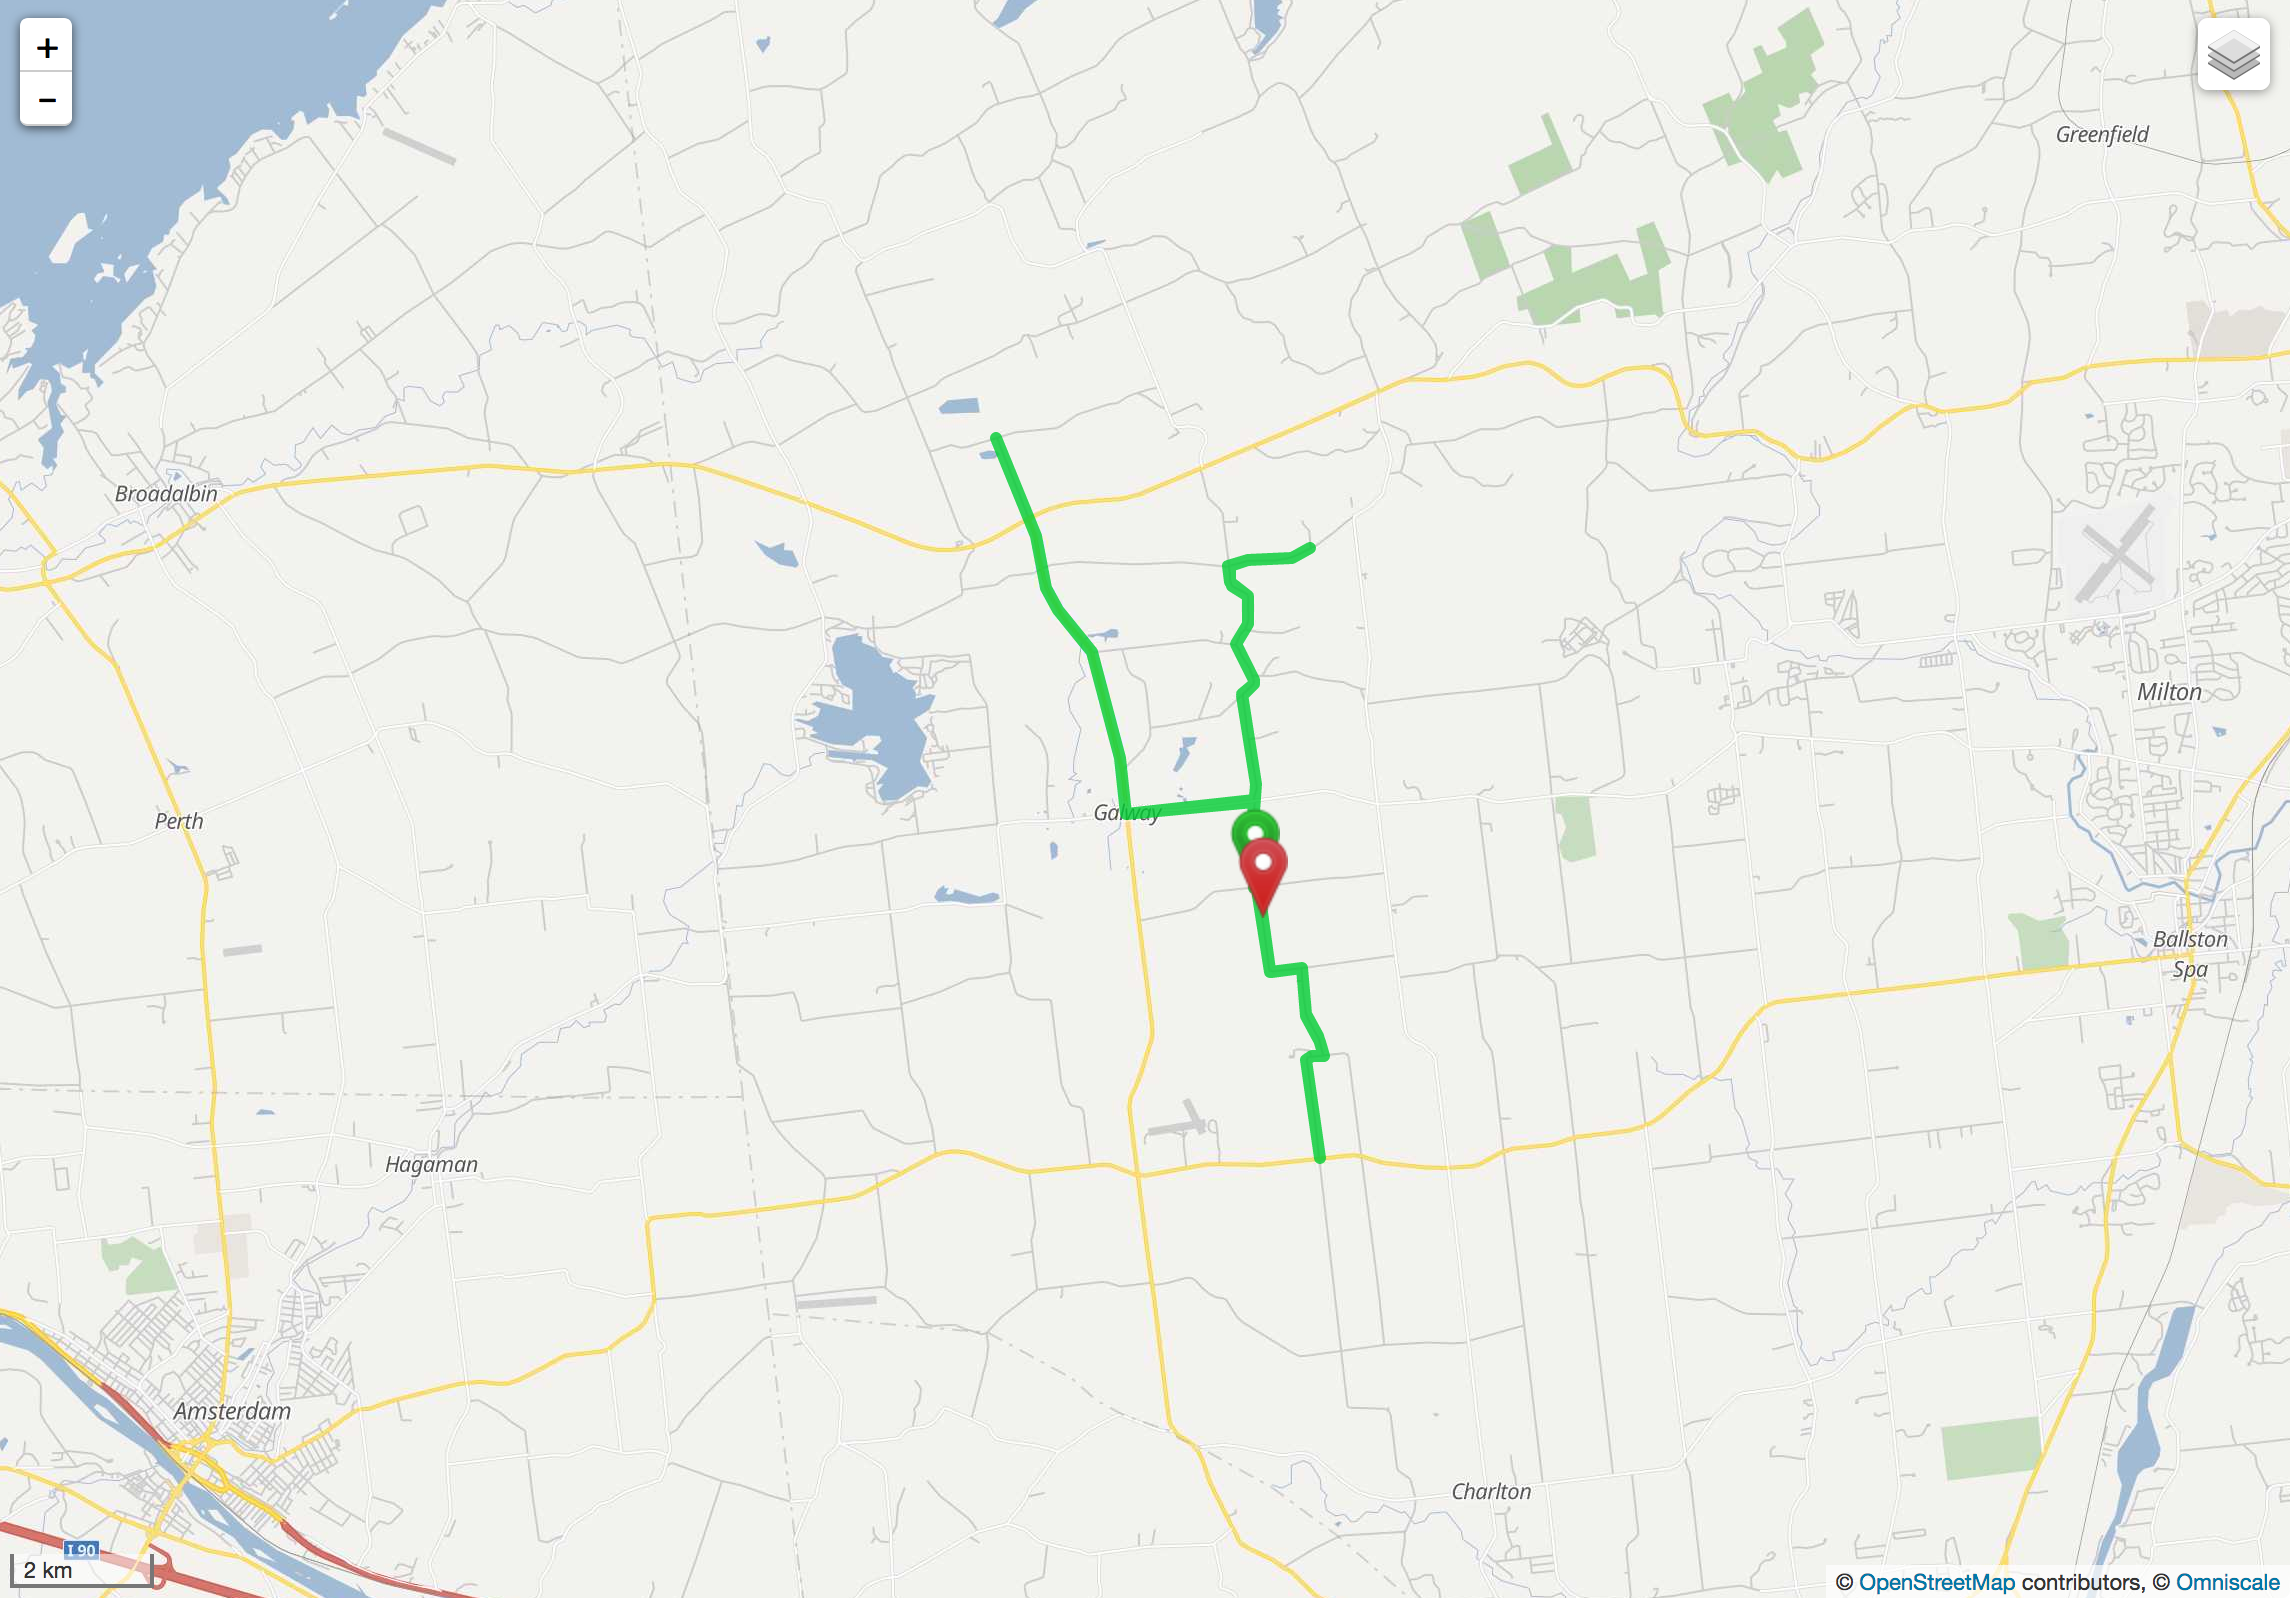
\includegraphics[width=\paperwidth]{figs/ls-route3}}
\caption{Route with excess backtracking by Geometric Algorithm.}
\end{figure}    
\end{frame}

\begin{frame}{Geometric Algorithm \cite{lu2015arc}}
    Limitations:
    \begin{itemize}
        \item Does not avoid backtracking.
        \item Tries to hit budget exactly.
        \item Shortest path not necessarily preferable.
        \item Does not penalize turns. 
    \end{itemize}
    \vspace{0.3cm}
    We designed and implemented variants:
    \begin{itemize}
        \item Avoid backtracking when gluing together attractive arcs.
        \item Don't use full budget when generating paths.
        \item Change which attractive arcs are considered.
    \end{itemize}
    
\end{frame}

%
% VVA
%
\section{Results}
\begin{frame}{Results: DFS \cite{verbeeck2014extension}}
\begin{center}
\begin{figure}
\tikzsetnextfilename{vva_graph}
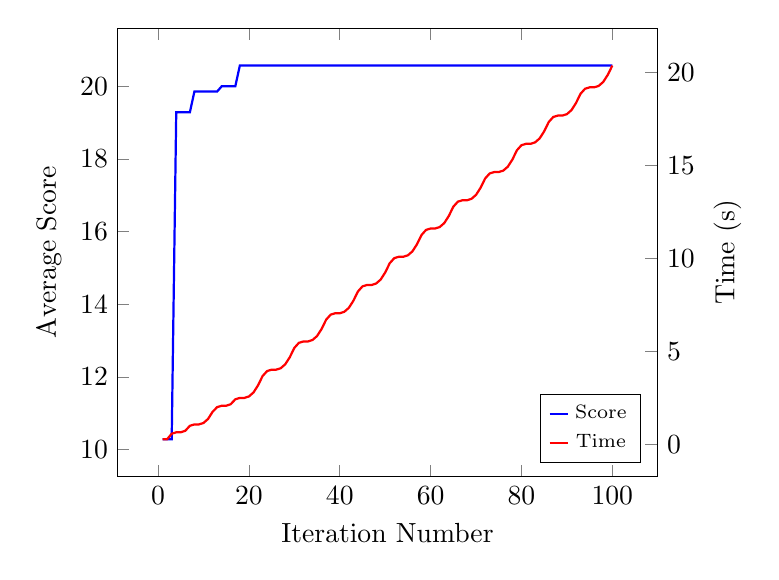
\begin{tikzpicture}
\begin{axis}[
    xlabel={Iteration Number},
    ylabel={Average Score},
    axis y line* = left,
]
\addplot[
    color=blue,
    style={thick}
    ]
    coordinates {
    (1, 10.285714000000002)(2, 10.285714000000002)(3, 10.285714000000002)(4, 19.285713999999995)(5, 19.285713999999995)(6, 19.285713999999995)(7, 19.285713999999995)(8, 19.857142999999997)(9, 19.857142999999997)(10, 19.857142999999997)(11, 19.857142999999997)(12, 19.857142999999997)(13, 19.857142999999997)(14, 20.0)(15, 20.0)(16, 20.0)(17, 20.0)(18, 20.571429000000002)(19, 20.571429000000002)(20, 20.571429000000002)(21, 20.571429000000002)(22, 20.571429000000002)(23, 20.571429000000002)(24, 20.571429000000002)(25, 20.571429000000002)(26, 20.571429000000002)(27, 20.571429000000002)(28, 20.571429000000002)(29, 20.571429000000002)(30, 20.571429000000002)(31, 20.571429000000002)(32, 20.571429000000002)(33, 20.571429000000002)(34, 20.571429000000002)(35, 20.571429000000002)(36, 20.571429000000002)(37, 20.571429000000002)(38, 20.571429000000002)(39, 20.571429000000002)(40, 20.571429000000002)(41, 20.571429000000002)(42, 20.571429000000002)(43, 20.571429000000002)(44, 20.571429000000002)(45, 20.571429000000002)(46, 20.571429000000002)(47, 20.571429000000002)(48, 20.571429000000002)(49, 20.571429000000002)(50, 20.571429000000002)(51, 20.571429000000002)(52, 20.571429000000002)(53, 20.571429000000002)(54, 20.571429000000002)(55, 20.571429000000002)(56, 20.571429000000002)(57, 20.571429000000002)(58, 20.571429000000002)(59, 20.571429000000002)(60, 20.571429000000002)(61, 20.571429000000002)(62, 20.571429000000002)(63, 20.571429000000002)(64, 20.571429000000002)(65, 20.571429000000002)(66, 20.571429000000002)(67, 20.571429000000002)(68, 20.571429000000002)(69, 20.571429000000002)(70, 20.571429000000002)(71, 20.571429000000002)(72, 20.571429000000002)(73, 20.571429000000002)(74, 20.571429000000002)(75, 20.571429000000002)(76, 20.571429000000002)(77, 20.571429000000002)(78, 20.571429000000002)(79, 20.571429000000002)(80, 20.571429000000002)(81, 20.571429000000002)(82, 20.571429000000002)(83, 20.571429000000002)(84, 20.571429000000002)(85, 20.571429000000002)(86, 20.571429000000002)(87, 20.571429000000002)(88, 20.571429000000002)(89, 20.571429000000002)(90, 20.571429000000002)(91, 20.571429000000002)(92, 20.571429000000002)(93, 20.571429000000002)(94, 20.571429000000002)(95, 20.571429000000002)(96, 20.571429000000002)(97, 20.571429000000002)(98, 20.571429000000002)(99, 20.571429000000002)(100, 20.571429000000002)
    }; \label{vva-graph-score}
\end{axis}

\begin{axis}[
    ylabel near ticks, yticklabel pos=right,
    ylabel={Time (s)},
    legend pos = {south east},
    legend style={font=\scriptsize\selectfont,},
    legend image post style={scale=0.4},
    hide x axis,
    axis y line*=right,
]
\addlegendimage{/pgfplots/refstyle=vva-graph-score, blue,style=thick}\addlegendentry{Score}
\addplot[
    color=red,
    style={thick}
    ]
    coordinates {
    (1, 0.2917333333333334)(2, 0.29176666666666673)(3, 0.5858)(4, 0.6609333333333333)(5, 0.6610666666666667)(6, 0.7467333333333334)(7, 1.0115666666666667)(8, 1.0864333333333331)(9, 1.0864666666666665)(10, 1.1650333333333334)(11, 1.3789999999999998)(12, 1.7636999999999998)(13, 2.013966666666667)(14, 2.0892)(15, 2.0892333333333335)(16, 2.174633333333333)(17, 2.436166666666667)(18, 2.510466666666667)(19, 2.510666666666667)(20, 2.5889999999999995)(21, 2.801066666666668)(22, 3.182533333333334)(23, 3.682233333333333)(24, 3.954033333333333)(25, 4.028600000000001)(26, 4.0287)(27, 4.1070666666666655)(28, 4.3194)(29, 4.699933333333332)(30, 5.199533333333333)(31, 5.470866666666666)(32, 5.5452)(33, 5.5452666666666675)(34, 5.624333333333334)(35, 5.836266666666666)(36, 6.217033333333333)(37, 6.7157)(38, 6.987600000000002)(39, 7.061833333333332)(40, 7.061899999999999)(41, 7.1415333333333315)(42, 7.353433333333334)(43, 7.734533333333334)(44, 8.233466666666665)(45, 8.506400000000003)(46, 8.580833333333334)(47, 8.580933333333336)(48, 8.659733333333334)(49, 8.871833333333337)(50, 9.253266666666665)(51, 9.751666666666667)(52, 10.024299999999998)(53, 10.098466666666667)(54, 10.098533333333332)(55, 10.177433333333335)(56, 10.390366666666665)(57, 10.771333333333333)(58, 11.270299999999999)(59, 11.543000000000001)(60, 11.617333333333333)(61, 11.6174)(62, 11.696566666666666)(63, 11.908366666666666)(64, 12.2895)(65, 12.789266666666668)(66, 13.0608)(67, 13.135299999999997)(68, 13.135433333333332)(69, 13.21386666666667)(70, 13.426033333333333)(71, 13.807233333333333)(72, 14.306100000000002)(73, 14.577566666666668)(74, 14.652299999999999)(75, 14.652333333333331)(76, 14.730900000000002)(77, 14.9427)(78, 15.323200000000003)(79, 15.822933333333335)(80, 16.095499999999998)(81, 16.169666666666664)(82, 16.169733333333333)(83, 16.248000000000005)(84, 16.46013333333333)(85, 16.840999999999998)(86, 17.340199999999996)(87, 17.6128)(88, 17.687133333333335)(89, 17.6872)(90, 17.765599999999996)(91, 17.97813333333334)(92, 18.359599999999997)(93, 18.859233333333336)(94, 19.13076666666666)(95, 19.20533333333333)(96, 19.205433333333335)(97, 19.283900000000003)(98, 19.49656666666667)(99, 19.876966666666664)(100, 20.375200000000003)
    };
\addlegendentry{Time}
\end{axis}
\end{tikzpicture}
\caption{Route generation with DFS Algorithm.}
\end{figure}
\end{center}
\end{frame}

%
% LS - No Mins
%
\begin{frame}{Results: Geometric \cite{lu2015arc}}
\begin{center}
\begin{figure}
\tikzsetnextfilename{ls_graph_no_mins}
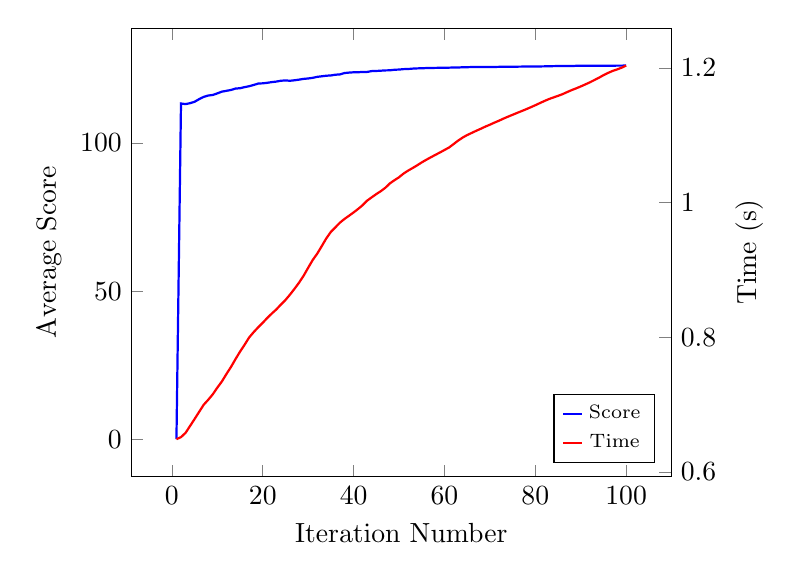
\begin{tikzpicture}
\begin{axis}[
    xlabel={Iteration Number},
    ylabel={Average Score},
    axis y line*=left,
]
\addplot[
    color=blue,
    style={thick}
    ]
    coordinates {
    (1, 0.0)(2, 113.34085713)(3, 113.13285712599999)(4, 113.44114284799998)(5, 113.93628571399998)(6, 114.81199999799999)(7, 115.57171428)(8, 116.03714285200002)(9, 116.21742857400004)(10, 116.75828571200002)(11, 117.34199999800002)(12, 117.62028572600003)(13, 117.90257142599998)(14, 118.38199999799997)(15, 118.49800000800002)(16, 118.87257143600002)(17, 119.17714285400002)(18, 119.595142854)(19, 120.06771428800003)(20, 120.15371428800005)(21, 120.32999999600001)(22, 120.57085713200001)(23, 120.74171428200002)(24, 121.02314285599999)(25, 121.13028571000001)(26, 121.01771428200004)(27, 121.18200000000006)(28, 121.40228571800006)(29, 121.65542857000004)(30, 121.78571428800005)(31, 122.01171428800005)(32, 122.33885715000004)(33, 122.52714286600006)(34, 122.72000000600008)(35, 122.80971429600008)(36, 123.05714286400008)(37, 123.16771428800007)(38, 123.62971428600007)(39, 123.77200000600007)(40, 123.87800000400006)(41, 123.90342857600005)(42, 123.98314286600005)(43, 124.01000000400006)(44, 124.27828572000006)(45, 124.32771429200007)(46, 124.41657144000008)(47, 124.51428572000006)(48, 124.54714286600007)(49, 124.73714286200006)(50, 124.80000001000005)(51, 124.94600001000006)(52, 124.98685715800009)(53, 125.11514287000007)(54, 125.19685715600005)(55, 125.23228572800006)(56, 125.30514287000005)(57, 125.34428572800006)(58, 125.36542858400007)(59, 125.39057143800002)(60, 125.43857144000006)(61, 125.44371429600005)(62, 125.48485715400007)(63, 125.50114286800006)(64, 125.56828572000002)(65, 125.60200000800003)(66, 125.64457143800003)(67, 125.64514286800004)(68, 125.64914286600003)(69, 125.66685715000004)(70, 125.67714286600004)(71, 125.67857143800003)(72, 125.71485714800004)(73, 125.72800000600003)(74, 125.74028572000005)(75, 125.76600000800005)(76, 125.77857143800003)(77, 125.79800000800003)(78, 125.82314286800003)(79, 125.82514287000004)(80, 125.85000000800004)(81, 125.85857143600005)(82, 125.88200001000003)(83, 125.91914287200004)(84, 125.95828572800004)(85, 125.97914286800004)(86, 125.99742858400003)(87, 125.96428572600004)(88, 125.99171429800005)(89, 126.06000001000005)(90, 126.05857143800004)(91, 126.07828572400004)(92, 126.06685715400006)(93, 126.06914286600005)(94, 126.08457143800005)(95, 126.09314286800006)(96, 126.10171429600005)(97, 126.11114286600004)(98, 126.12600001200006)(99, 126.13314286800005)(100, 126.13628572800008)    };
    \label{ls-graph-no-mins}
\end{axis}

\begin{axis}[
    ylabel near ticks, yticklabel pos=right,
    ylabel={Time (s)},
    legend pos = {south east},
    legend style={font=\scriptsize\selectfont,},
    legend image post style={scale=0.4},
    hide x axis,
    axis y line*=right,
]
\addlegendimage{/pgfplots/refstyle=ls-graph-no-mins, blue,style=thick}\addlegendentry{Score}
\addplot[
    color=red,
    style={thick}
    ]
    coordinates {
    (1, 0.6484239999999999)(2, 0.6514860000000001)(3, 0.6578380000000007)(4, 0.6680680000000001)(5, 0.6785079999999996)(6, 0.6890759999999995)(7, 0.6996239999999991)(8, 0.7070420000000003)(9, 0.715154)(10, 0.7250499999999999)(11, 0.7341979999999994)(12, 0.7452499999999993)(13, 0.7557399999999997)(14, 0.7674019999999997)(15, 0.7785680000000005)(16, 0.7887460000000001)(17, 0.7995779999999989)(18, 0.8075000000000003)(19, 0.8147479999999998)(20, 0.8213840000000001)(21, 0.8286939999999998)(22, 0.8352119999999998)(23, 0.8413279999999996)(24, 0.8485659999999997)(25, 0.8553300000000001)(26, 0.8632959999999997)(27, 0.8720539999999996)(28, 0.8811159999999999)(29, 0.891386)(30, 0.9032420000000009)(31, 0.9147340000000005)(32, 0.9242560000000001)(33, 0.9354919999999995)(34, 0.9469479999999997)(35, 0.9565439999999996)(36, 0.9633579999999996)(37, 0.9702779999999993)(38, 0.9757819999999988)(39, 0.9805380000000005)(40, 0.9854359999999998)(41, 0.990646)(42, 0.9962919999999997)(43, 1.0030420000000002)(44, 1.0079259999999992)(45, 1.0126820000000003)(46, 1.0170699999999995)(47, 1.0221019999999996)(48, 1.0286639999999991)(49, 1.033318)(50, 1.0376960000000004)(51, 1.0431919999999992)(52, 1.0475559999999993)(53, 1.0514260000000002)(54, 1.0554539999999997)(55, 1.059778)(56, 1.0636680000000003)(57, 1.0673420000000002)(58, 1.0709620000000004)(59, 1.0744840000000015)(60, 1.0781799999999988)(61, 1.0818700000000003)(62, 1.0869339999999992)(63, 1.0921120000000006)(64, 1.0966420000000012)(65, 1.1004280000000002)(66, 1.1035620000000004)(67, 1.1067599999999997)(68, 1.1097819999999996)(69, 1.112928000000001)(70, 1.1158099999999995)(71, 1.118867999999999)(72, 1.1217159999999993)(73, 1.124844000000001)(74, 1.1277419999999994)(75, 1.130534)(76, 1.1333380000000004)(77, 1.1360500000000007)(78, 1.1388140000000002)(79, 1.141731999999999)(80, 1.1447419999999997)(81, 1.1478940000000009)(82, 1.1510079999999994)(83, 1.1539019999999995)(84, 1.1563140000000003)(85, 1.1586559999999997)(86, 1.161204)(87, 1.164269999999999)(88, 1.1671879999999992)(89, 1.1698299999999988)(90, 1.1726500000000013)(91, 1.1756340000000016)(92, 1.17872)(93, 1.182118000000001)(94, 1.1855639999999994)(95, 1.189377999999999)(96, 1.1926920000000003)(97, 1.195632)(98, 1.1979300000000002)(99, 1.200514)(100, 1.203648)
    };
    \addlegendentry{Time}
\end{axis}
\end{tikzpicture}
\caption{Route generation with Geometric Algorithm.}
\end{figure}
\end{center}
\end{frame}

%
% LS - Fixed budget percent
%
\begin{frame}{Results: Geometric + (Budget allowance)}
\begin{center}
\begin{figure}
\tikzsetnextfilename{ls_graph_fixed_percent}
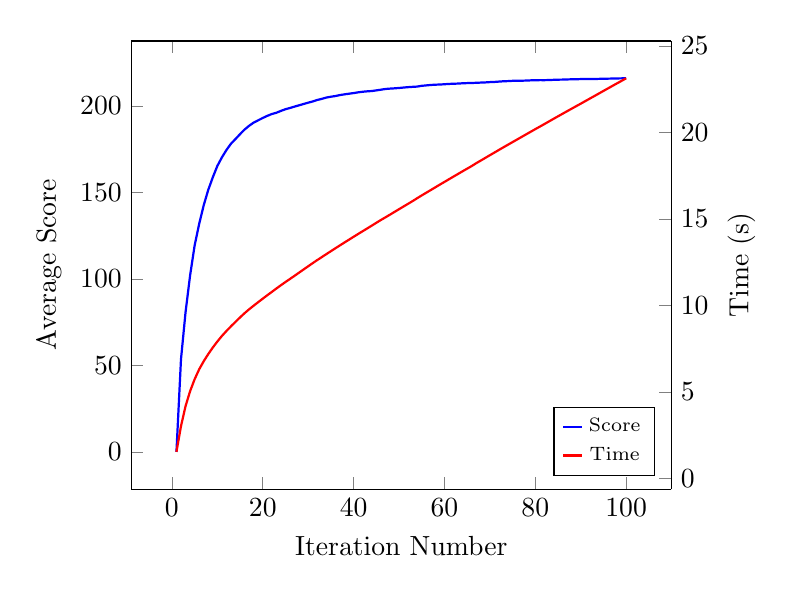
\begin{tikzpicture}
\begin{axis}[
    xlabel={Iteration Number},
    ylabel={Average Score},
    axis y line*=left,
]
\addplot[
    color=blue,
    style={thick}
    ]
    coordinates {
    (1, 0.0)(2, 53.54485713999996)(3, 80.64771426999998)(4, 101.89742856599999)(5, 119.24199999600005)(6, 131.7399999739999)(7, 142.49685714199998)(8, 151.40599999599996)(9, 158.63885713799996)(10, 165.21742856799995)(11, 170.16171427199995)(12, 174.43285714399994)(13, 178.07999998999992)(14, 180.800285716)(15, 183.61457141399993)(16, 186.26914284999992)(17, 188.46057141599994)(18, 190.29114284399992)(19, 191.62828570799994)(20, 192.95685712799994)(21, 194.193142852)(22, 195.24485713199996)(23, 195.97799998599993)(24, 197.05199998999993)(25, 198.02257142199994)(26, 198.73742857399992)(27, 199.54057142199986)(28, 200.28571427799992)(29, 201.04628571999996)(30, 201.802)(31, 202.500000006)(32, 203.36428572000003)(33, 204.00085713799996)(34, 204.760571426)(35, 205.24142858200003)(36, 205.6391428539999)(37, 206.19714284999995)(38, 206.61485715000003)(39, 206.988857142)(40, 207.34314286400004)(41, 207.77142857600006)(42, 208.11285714600007)(43, 208.35485713399993)(44, 208.52971428200001)(45, 208.90342856800004)(46, 209.292571424)(47, 209.70971428199994)(48, 209.92285714800002)(49, 210.08914287000005)(50, 210.28828572400005)(51, 210.54571429800006)(52, 210.77085714199998)(53, 210.95171428199998)(54, 211.105428574)(55, 211.53742856799997)(56, 211.78028569999992)(57, 212.03142856799997)(58, 212.196285712)(59, 212.28257142199996)(60, 212.45714285399998)(61, 212.634571428)(62, 212.74742856999998)(63, 212.833714288)(64, 213.01599999799998)(65, 213.10799999399995)(66, 213.18457142399996)(67, 213.27800000400003)(68, 213.409714288)(69, 213.506571434)(70, 213.68800000599998)(71, 213.78028570999996)(72, 213.98228570999996)(73, 214.16999999999996)(74, 214.268)(75, 214.41742856799996)(76, 214.44857142799998)(77, 214.49771428199995)(78, 214.57571428599996)(79, 214.69828571600002)(80, 214.75171428399997)(81, 214.82599999599998)(82, 214.80885713599992)(83, 214.87228570999997)(84, 214.9914285639999)(85, 215.09542856999997)(86, 215.13257142999998)(87, 215.23628570999998)(88, 215.29799999599996)(89, 215.35085713799995)(90, 215.43199999799995)(91, 215.43171428599996)(92, 215.45342856799996)(93, 215.508285714)(94, 215.552571428)(95, 215.63142857)(96, 215.68257142799996)(97, 215.72771428599998)(98, 215.81257142399997)(99, 215.85142857)(100, 215.87714286)    }; \label{ls-graph-budget-percent}
\end{axis}

\begin{axis}[
    ylabel near ticks, yticklabel pos=right,
    ylabel={Time (s)},
    legend pos = {south east},
    legend style={font=\scriptsize\selectfont,},
    legend image post style={scale=0.4},
    hide x axis,
    axis y line*=right,
]
\addlegendimage{/pgfplots/refstyle=ls-graph-budget-percent, blue,style=thick}\addlegendentry{Score}
\addplot[
    color=red,
    style={thick}
    ]
    coordinates {
(1, 1.5404639999999994)(2, 3.030628000000002)(3, 4.181223999999998)(4, 5.045037999999998)(5, 5.736461999999995)(6, 6.3113119999999965)(7, 6.778498000000003)(8, 7.190831999999996)(9, 7.569965999999998)(10, 7.915543999999994)(11, 8.236798000000002)(12, 8.523962000000001)(13, 8.794169999999998)(14, 9.055248)(15, 9.309724000000001)(16, 9.554674000000006)(17, 9.779929999999986)(18, 9.987127999999995)(19, 10.193661999999996)(20, 10.392640000000007)(21, 10.591159999999993)(22, 10.784546000000004)(23, 10.979709999999994)(24, 11.170064000000004)(25, 11.35469600000001)(26, 11.533738)(27, 11.714087999999997)(28, 11.897320000000015)(29, 12.082166000000004)(30, 12.263632000000001)(31, 12.447411999999998)(32, 12.622923999999996)(33, 12.796045999999993)(34, 12.965997999999995)(35, 13.135870000000008)(36, 13.306078000000007)(37, 13.472791999999991)(38, 13.638972000000006)(39, 13.803319999999998)(40, 13.968022000000007)(41, 14.130964)(42, 14.29088800000001)(43, 14.449906000000002)(44, 14.611660000000006)(45, 14.775492000000003)(46, 14.936703999999986)(47, 15.089251999999998)(48, 15.244979999999991)(49, 15.402916000000017)(50, 15.560572)(51, 15.718013999999997)(52, 15.874412000000001)(53, 16.03148999999999)(54, 16.196709999999992)(55, 16.358036000000002)(56, 16.514659999999985)(57, 16.669493999999993)(58, 16.827065999999988)(59, 16.983418000000004)(60, 17.13686600000002)(61, 17.292453999999996)(62, 17.44666399999999)(63, 17.599136)(64, 17.753107999999994)(65, 17.903282000000008)(66, 18.05397600000001)(67, 18.219918000000025)(68, 18.371512)(69, 18.52604999999999)(70, 18.679675999999997)(71, 18.833196000000015)(72, 18.986647999999978)(73, 19.138872000000006)(74, 19.289375999999983)(75, 19.438833999999996)(76, 19.587687999999982)(77, 19.73728600000002)(78, 19.88783400000001)(79, 20.036580000000015)(80, 20.185724000000018)(81, 20.331694000000006)(82, 20.47928)(83, 20.629487999999995)(84, 20.77885399999999)(85, 20.92689000000002)(86, 21.074596000000014)(87, 21.221957999999994)(88, 21.367570000000015)(89, 21.512194000000026)(90, 21.656795999999996)(91, 21.80439799999998)(92, 21.951017999999987)(93, 22.098104000000017)(94, 22.244324000000017)(95, 22.39271799999999)(96, 22.540094000000003)(97, 22.686846000000035)(98, 22.832402000000023)(99, 22.977423999999996)(100, 23.122468000000012)
    };
    \addlegendentry{Time}
\end{axis}
\end{tikzpicture}
\caption{Geometric Algorithm with 50\% budget allowance.}
\end{figure}
\end{center}
\end{frame}

%
% LS - Incremental budget
%
%\begin{frame}{Experimental Results}
%\begin{center}
%\begin{figure}
%\tikzsetnextfilename{ls_graph_incremental_budget}
%\begin{tikzpicture}
%\begin{axis}[
%    xlabel={Iteration Number},
%    ylabel={Average Score},
%    axis y line*=left,
%]
%\addplot[
%    color=blue,
%    style={thick}
%    ]
%    coordinates {
%    (1, 0.0)(2, 1.1428570000000005)(3, 1.1428570000000005)(4, 1.1428570000000005)(5, 1.1428570000000005)(6, 1.1428570000000005)(7, 1.1428570000000005)(8, 1.1428570000000005)(9, 1.1428570000000005)(10, 1.1428570000000005)(11, 1.1428570000000005)(12, 1.1428570000000005)(13, 1.1428570000000005)(14, 1.1428570000000005)(15, 1.1428570000000005)(16, 1.1428570000000005)(17, 5.414857216000013)(18, 5.883428504000005)(19, 7.108571458000036)(20, 8.633714298000056)(21, 10.141142892000053)(22, 14.233714148000068)(23, 18.419428538000034)(24, 23.897142851999998)(25, 29.962285719999997)(26, 36.25942857399999)(27, 42.79657141400004)(28, 49.28685713600003)(29, 55.87428571799998)(30, 62.594857146000074)(31, 69.05657141000003)(32, 75.74514283599999)(33, 82.16628570399997)(34, 88.19942858400005)(35, 94.41657141599998)(36, 100.50971428599993)(37, 106.36685715200004)(38, 111.99485714600002)(39, 117.22285712199994)(40, 122.11714287400005)(41, 127.04571427599996)(42, 131.70571429400007)(43, 136.14285716400008)(44, 140.63485713199998)(45, 144.7988571219999)(46, 148.75199999800006)(47, 152.506285748)(48, 156.156571422)(49, 159.60799998799996)(50, 163.16971427399992)(51, 166.60685713199996)(52, 170.00628570399985)(53, 173.2828571360001)(54, 176.43142857199993)(55, 179.56685715000003)(56, 182.66057143800003)(57, 185.82228570800004)(58, 188.970285716)(59, 192.10228572400007)(60, 195.13942856799997)(61, 198.23371428800002)(62, 201.037142862)(63, 203.84628569999987)(64, 206.54171426999986)(65, 209.2325714139999)(66, 211.85657141999994)(67, 214.469714276)(68, 216.9542857280001)(69, 219.33028571600002)(70, 221.7485714540002)(71, 224.096000012)(72, 226.6600000100001)(73, 229.07485714199996)(74, 231.38742855799984)(75, 233.646285726)(76, 235.93485715600005)(77, 238.102285714)(78, 240.25085715600008)(79, 242.398857144)(80, 244.50571429199994)(81, 246.72057142399998)(82, 248.94114285800003)(83, 251.08000001000002)(84, 253.11885713799998)(85, 255.17085714799998)(86, 257.21314285399995)(87, 259.245714286)(88, 261.304571434)(89, 263.21885714199993)(90, 265.01542858000005)(91, 266.925142856)(92, 268.7880000200001)(93, 270.65600001800016)(94, 272.484000006)(95, 274.35314285399994)(96, 276.05942857199994)(97, 277.7245714420001)(98, 279.333714294)(99, 281.05542859800016)(100, 282.66971429800003)    }; \label{ls-graph-incremental}
%\end{axis}
%
%\begin{axis}[
%    ylabel near ticks, yticklabel pos=right,
%    ylabel={Time (s)},
%    legend pos = {south east},
%    legend style={font=\scriptsize\selectfont},
%    legend image post style={scale=0.4},
%    hide x axis,
%    axis y line*=right,
%]
%\addlegendimage{/pgfplots/refstyle=ls-graph-incremental, blue,style=thick}\addlegendentry{Score}
%\addplot[
%    color=red,
%    style={thick}
%    ]
%    coordinates {
%(1, 0.6553780000000007)(2, 0.8145339999999994)(3, 0.9736880000000008)(4, 1.133602000000002)(5, 1.2937079999999974)(6, 1.454020000000001)(7, 1.6141880000000022)(8, 1.7739779999999983)(9, 1.9332999999999967)(10, 2.0923160000000007)(11, 2.2512020000000015)(12, 2.4099279999999994)(13, 2.569098000000002)(14, 2.7278939999999987)(15, 2.8868360000000006)(16, 3.565115999999996)(17, 4.133447999999998)(18, 4.9078959999999965)(19, 5.931039999999992)(20, 7.170333999999998)(21, 9.014160000000002)(22, 11.527971999999993)(23, 14.976956000000005)(24, 19.294753999999976)(25, 24.49373600000001)(26, 30.447487999999986)(27, 37.11408799999997)(28, 44.22119600000003)(29, 51.59153)(30, 58.79706399999997)(31, 65.64260600000003)(32, 71.93420800000005)(33, 77.40983799999997)(34, 82.15846599999993)(35, 86.08474399999994)(36, 89.32948999999992)(37, 92.03269800000001)(38, 94.244002)(39, 96.03647800000007)(40, 97.55355000000013)(41, 98.82415200000004)(42, 99.90436400000003)(43, 100.83597400000004)(44, 101.64726799999995)(45, 102.37428600000004)(46, 103.01933199999989)(47, 103.60660799999991)(48, 104.15785799999988)(49, 104.66250599999998)(50, 105.14375800000002)(51, 105.593072)(52, 106.01980600000016)(53, 106.42931400000003)(54, 106.83500600000005)(55, 107.23226799999995)(56, 107.62728399999997)(57, 108.01994)(58, 108.39690200000013)(59, 108.75836800000006)(60, 109.11838199999985)(61, 109.46851800000012)(62, 109.81155199999996)(63, 110.13977800000008)(64, 110.45737799999996)(65, 110.76974799999998)(66, 111.07706600000006)(67, 111.38328600000004)(68, 111.68629599999991)(69, 111.99076400000007)(70, 112.29828000000003)(71, 112.60102600000003)(72, 112.9068540000001)(73, 113.20118799999997)(74, 113.49045799999999)(75, 113.77756000000008)(76, 114.05764600000002)(77, 114.32137399999995)(78, 114.58435000000006)(79, 114.85938999999998)(80, 115.1284100000001)(81, 115.39673399999998)(82, 115.65732200000006)(83, 115.90934999999989)(84, 116.15202600000002)(85, 116.38925200000013)(86, 116.61209599999992)(87, 116.83666599999987)(88, 117.06390800000005)(89, 117.29110199999995)(90, 117.52334999999998)(91, 117.75103200000001)(92, 117.97224800000004)(93, 118.17810599999993)(94, 118.37594199999995)(95, 118.56767599999992)(96, 118.76787799999998)(97, 118.96026999999984)(98, 119.14996399999991)(99, 119.3383299999999)(100, 119.52416600000016)    };
%\addlegendentry{Time}
%\end{axis}
%\end{tikzpicture}
%\caption{Algorithm 2 with incremental budget.}
%\end{figure}
%\end{center}
%\end{frame}



%
% LS - With mins
%
%\begin{frame}{Experimental Results}
%\begin{center}
%\begin{figure}
%\tikzsetnextfilename{ls_graph_with_mins}
%\begin{tikzpicture}
%\begin{axis}[
%    xlabel={Iteration Number},
%    ylabel={Average Score},
%    axis y line*=left,
%]
%\addplot[
%    color=blue,
%    style={thick}
%    ]
%    coordinates {
%    (1, 0.0)(2, 49.93028571600001)(3, 49.94514285600001)(4, 49.93600000200001)(5, 49.92400000200001)(6, 49.91771428800001)(7, 49.912000002000006)(8, 49.912000002000006)(9, 49.89714286000001)(10, 49.892571432000004)(11, 49.89200000200001)(12, 49.869714288000004)(13, 49.87857143)(14, 49.87857143)(15, 49.87857143)(16, 49.87857143)(17, 49.87857143)(18, 49.87857143)(19, 49.87857143)(20, 49.87857143)(21, 49.87857143)(22, 49.83171428600001)(23, 49.83457143000001)(24, 49.78800000200002)(25, 49.843714286000015)(26, 49.843714286000015)(27, 49.84685714400002)(28, 49.850285716000016)(29, 49.850285716000016)(30, 49.850285716000016)(31, 49.850285716000016)(32, 49.850285716000016)(33, 49.850285716000016)(34, 49.850285716000016)(35, 49.850285716000016)(36, 49.85314285800001)(37, 49.85314285800001)(38, 49.85314285800001)(39, 49.85314285800001)(40, 49.85314285800001)(41, 49.85314285800001)(42, 49.85314285800001)(43, 49.85314285800001)(44, 49.85314285800001)(45, 49.85314285800001)(46, 49.85314285800001)(47, 49.85314285800001)(48, 49.85314285800001)(49, 49.85314285800001)(50, 49.85314285800001)(51, 49.85314285800001)(52, 49.85314285800001)(53, 49.85314285800001)(54, 49.85314285800001)(55, 49.85314285800001)(56, 49.85314285800001)(57, 49.85314285800001)(58, 49.85314285800001)(59, 49.85314285800001)(60, 49.85314285800001)(61, 49.85314285800001)(62, 49.85314285800001)(63, 49.85314285800001)(64, 49.85314285800001)(65, 49.85314285800001)(66, 49.85314285800001)(67, 49.85314285800001)(68, 49.85314285800001)(69, 49.85314285800001)(70, 49.85314285800001)(71, 49.85314285800001)(72, 49.85314285800001)(73, 49.85314285800001)(74, 49.85314285800001)(75, 49.85314285800001)(76, 49.85314285800001)(77, 49.85314285800001)(78, 49.85314285800001)(79, 49.85314285800001)(80, 49.85314285800001)(81, 49.85314285800001)(82, 49.85314285800001)(83, 49.85314285800001)(84, 49.85314285800001)(85, 49.85314285800001)(86, 49.85314285800001)(87, 49.85314285800001)(88, 49.85314285800001)(89, 49.85314285800001)(90, 49.85314285800001)(91, 49.85314285800001)(92, 49.85314285800001)(93, 49.85314285800001)(94, 49.85314285800001)(95, 49.85314285800001)(96, 49.85314285800001)(97, 49.85314285800001)(98, 49.85314285800001)(99, 49.85314285800001)(100, 49.85314285800001)    };
%    \label{ls-graph-arc-restriction}
%\end{axis}
%
%\begin{axis}[
%    ylabel near ticks, yticklabel pos=right,
%    ylabel={Time (s)},
%    legend pos = {south east},
%    legend style={font=\scriptsize\selectfont},
%    legend image post style={scale=0.4},
%    hide x axis,
%    axis y line*=right,
%]
%\addlegendimage{/pgfplots/refstyle=ls-graph-arc-restriction, blue,style=thick}\addlegendentry{Score}
%\addplot[
%    color=red,
%    style={thick}
%    ]
%    coordinates {
%    (1, 0.06131999999999988)(2, 0.061715999999999785)(3, 0.06209799999999986)(4, 0.06246599999999992)(5, 0.062836)(6, 0.06320000000000005)(7, 0.0635720000000001)(8, 0.06393000000000006)(9, 0.06433000000000004)(10, 0.06464600000000001)(11, 0.06511599999999995)(12, 0.06557400000000002)(13, 0.06595200000000004)(14, 0.06635200000000008)(15, 0.0667160000000001)(16, 0.06710400000000008)(17, 0.06749200000000007)(18, 0.06787600000000006)(19, 0.06827400000000008)(20, 0.0686620000000001)(21, 0.06906200000000014)(22, 0.06944600000000016)(23, 0.06996400000000015)(24, 0.07045000000000008)(25, 0.07085200000000011)(26, 0.07127200000000013)(27, 0.07164800000000023)(28, 0.07201600000000023)(29, 0.07240000000000016)(30, 0.07278600000000014)(31, 0.07319400000000009)(32, 0.07353600000000013)(33, 0.07393200000000018)(34, 0.07431600000000017)(35, 0.0747200000000002)(36, 0.07507000000000025)(37, 0.0754680000000002)(38, 0.07586200000000018)(39, 0.0762320000000001)(40, 0.07661400000000015)(41, 0.07700400000000017)(42, 0.07736200000000024)(43, 0.07775000000000025)(44, 0.07812400000000023)(45, 0.07850200000000024)(46, 0.0789020000000002)(47, 0.07929000000000017)(48, 0.07971800000000012)(49, 0.0800880000000001)(50, 0.08045600000000012)(51, 0.08088600000000024)(52, 0.08126800000000024)(53, 0.08166600000000022)(54, 0.0820400000000002)(55, 0.08241200000000015)(56, 0.08277800000000017)(57, 0.08319200000000013)(58, 0.08358000000000014)(59, 0.08396200000000016)(60, 0.08435200000000012)(61, 0.08474600000000014)(62, 0.08514200000000008)(63, 0.08551200000000012)(64, 0.0858940000000001)(65, 0.08630000000000013)(66, 0.08669000000000017)(67, 0.08705600000000013)(68, 0.08742000000000014)(69, 0.08781400000000007)(70, 0.08819600000000011)(71, 0.08858400000000015)(72, 0.08894600000000018)(73, 0.08935600000000024)(74, 0.08971400000000021)(75, 0.09008600000000012)(76, 0.09048000000000009)(77, 0.09086000000000008)(78, 0.09123200000000006)(79, 0.09162600000000007)(80, 0.09200000000000015)(81, 0.09239200000000032)(82, 0.09279000000000025)(83, 0.09315200000000014)(84, 0.09356200000000005)(85, 0.09393400000000006)(86, 0.09428400000000008)(87, 0.09469600000000016)(88, 0.09507600000000016)(89, 0.09545600000000022)(90, 0.0958000000000002)(91, 0.09622000000000012)(92, 0.0965960000000001)(93, 0.09697600000000009)(94, 0.09739200000000009)(95, 0.09774800000000004)(96, 0.09816200000000007)(97, 0.09850800000000011)(98, 0.09890400000000006)(99, 0.09930000000000004)(100, 0.09965000000000003)
%    };
%\addlegendentry{Time}
%\end{axis}
%\end{tikzpicture}
%\caption{Algorithm 2 with attractive arc restrictions.}
%\end{figure}
%\end{center}
%\end{frame}

\begin{frame}{Conclusions}
    \begin{itemize}
        \item Spatial techniques definitely speed up ILS.
        \item Modifying budget over time greatly increases average score at a hefty time penalty.
        \item Attractive arc definition and data set matter a lot in algorithm performance.
    \end{itemize}
    
    \begin{center}
    \begin{figure}
    \begin{tabular}{|p{15em}|l|l|l|l|}
    \hline
    \textbf{Algorithm} & \textbf{Score} & \textbf{Time (s)} & \textbf{Ratio} \\
    \hline
    DFS & 20.57 & 20.37 & 1.00 \\
    \hline
    Geometric & 126.13 & 1.20 & 105.10 \\
    \hline
    Geometric + (Budget allowance) & 215.87 & 23.12 & 9.33 \\
    \hline
    Geometric + (Incremental budget) & 282.66 & 119.52 & 2.36 \\
    \hline
    Geometric + (Arc restrictions) & 49.85 & 0.09 & 553.88 \\
    \hline
    Geometric + (No backtracking) & 33.36 & 0.60 & 55.6 \\
    \hline
    Geometric + (Budget allowance) + (Arc restrictions) & 32.49 & 2.37 & 13.70 \\
    \hline
    \end{tabular}
    \caption{Algorithm performance of variants.}
    \end{figure}
    \end{center}
\end{frame}

\begin{frame}{Conclusions}
\begin{itemize}
    \item Using a smarter ILS cutoff strategy can save substantial time.
\end{itemize}
    \begin{center}
    \begin{figure}
    \begin{tabular}{|p{15em}|l|l|l|}
    \hline
    \textbf{Algorithm} & \textbf{Score} & \textbf{Time (s)} & \textbf{Ratio} \\
    \hline
    DFS & 19.28 & 1.01 & 19.08 \\
    \hline
    Geometric & 113.93 & 0.67 & 170.0 \\
    \hline
    Geometric + (Budget allowance) & 192.95 & 10.39 & 18.57 \\
    \hline
    Geometric + (Incremental budget) & 1.14 & 1.29 & 0.88 \\
    \hline
    Geometric + (Arc restrictions) & 49.92 & 0.06 & 832 \\
    \hline
    Geometric + (No backtracking) & 33.37 & 0.61 & 54.70 \\
    \hline
    Geometric + (Budget allowance) + (Arc restrictions) & 30.80 & 0.88 & 35 \\
    \hline
    \end{tabular}
    \caption{Algorithm performance of variants with score-cutoff.}
    \end{figure}
    \end{center}
\end{frame}


%\begin{frame}{Experimental Results}
%\begin{center}
%\begin{tikzpicture}
%\begin{axis}[
%    title={Score vs Iteration},
%    xlabel={Iteration Number},
%    ylabel={Average Score},
%    ymajorgrids=true,
%    grid style=dashed,
%    legend pos=outer north east,
%    legend style={font=\scriptsize\selectfont},
%    legend image post style={scale=0.4 },
%]
%\addplot[
%    color=blue,
%    style={thick}
%    ]
%    coordinates {
%    (1, 0.0)(2, 116.55828572199992)(3, 116.38857142799989)(4, 117.39571430199996)(5, 118.6271428559999)(6, 119.50142857999997)(7, 121.18400000199995)(8, 122.192285722)(9, 123.11057142799997)(10, 124.50742857600005)(11, 125.68400000800003)(12, 126.744000004)(13, 127.06342857799999)(14, 127.57857143399998)(15, 128.08971429)(16, 128.45485713799994)(17, 128.92571429199998)(18, 129.328000004)(19, 129.87514286399994)(20, 130.110571442)(21, 130.26371428399997)(22, 130.58314286200005)(23, 131.16257143400003)(24, 131.39485715400005)(25, 131.85028572200002)(26, 132.12885716000002)(27, 132.58085716000008)(28, 132.97400001400004)(29, 133.347714296)(30, 133.583714294)(31, 133.82371430200004)(32, 133.96600001200002)(33, 134.17371429599996)(34, 134.53800001000002)(35, 134.74085715800004)(36, 134.96628572800003)(37, 135.04714287000002)(38, 135.09542859000004)(39, 135.27457144400006)(40, 135.34228573200005)(41, 135.39428573000006)(42, 135.48228573000006)(43, 135.51685715400006)(44, 135.75657144200008)(45, 135.81600001600006)(46, 135.84942858800008)(47, 136.04371430000003)(48, 136.12628572600002)(49, 136.286000008)(50, 136.385142862)(51, 136.41371429000003)(52, 136.45428572200007)(53, 136.569142864)(54, 136.640285716)(55, 136.66799999799994)(56, 136.68485714800002)(57, 136.72057142999998)(58, 136.917428574)(59, 137.03942856999998)(60, 137.095428572)(61, 137.192857148)(62, 137.318857146)(63, 137.354571434)(64, 137.39400000199998)(65, 137.425428576)(66, 137.490571434)(67, 137.54171429200005)(68, 137.56028571800002)(69, 137.63885715200004)(70, 137.66971429000003)(71, 137.75428571600003)(72, 137.83571429000003)(73, 137.87285715000002)(74, 138.03057143400002)(75, 138.09400000600002)(76, 138.116571432)(77, 138.09600000600003)(78, 138.158000006)(79, 138.16142857600005)(80, 138.24285714800004)(81, 138.34828571800003)(82, 138.42257143199998)(83, 138.46171428800002)(84, 138.60371429000003)(85, 138.85914286000002)(86, 138.85285714600002)(87, 138.86657143400004)(88, 138.90200000800004)(89, 138.94171429200006)(90, 138.98914286000004)(91, 139.02828571800003)(92, 139.03200000400005)(93, 139.03371428800008)(94, 139.06342857400008)(95, 139.13971429000006)(96, 139.18771429200004)(97, 139.21628572200007)(98, 139.22771429400007)(99, 139.2057142940001)(100, 139.23114286600008)
%    };
%
%\addplot[
%    color=red,
%    style={thick}
%    ]
%    coordinates {
%    (1, 0.0)(2, 52.730285696000074)(3, 79.43800000200004)(4, 100.22571427799998)(5, 116.77685715400003)(6, 132.3271428820002)(7, 142.88771430000014)(8, 152.4165714420001)(9, 160.34542858400008)(10, 166.65085713800002)(11, 172.06514286799995)(12, 176.70171428800003)(13, 180.391714284)(14, 183.5240000180001)(15, 186.15057145000011)(16, 188.59200002400019)(17, 190.23742856399997)(18, 192.20200000199998)(19, 194.04971428400003)(20, 195.51885714400004)(21, 196.80114286000006)(22, 198.098285708)(23, 199.137999996)(24, 200.26114285)(25, 201.38999999)(26, 202.20771428200004)(27, 202.84371428800003)(28, 203.63342857800006)(29, 204.2922857240001)(30, 205.12457142199997)(31, 205.74742856399996)(32, 206.2042857019999)(33, 206.78028570399994)(34, 207.367142844)(35, 207.66828569799998)(36, 208.09628569399993)(37, 208.78771426399993)(38, 209.37742856600008)(39, 209.90857142800004)(40, 210.3785714380001)(41, 210.85199999399995)(42, 211.28257142799998)(43, 211.71028571200003)(44, 212.16714286000004)(45, 212.45485714800003)(46, 212.9565714400001)(47, 213.38600000800008)(48, 213.90457142600005)(49, 214.25399998799995)(50, 214.52028570399995)(51, 214.78371427599998)(52, 214.964857138)(53, 215.12314284399997)(54, 215.36199998599994)(55, 215.61114285400004)(56, 215.844857138)(57, 216.14885714400003)(58, 216.40371428)(59, 216.670285712)(60, 216.82914285400003)(61, 216.947428566)(62, 217.006285716)(63, 217.13914285800004)(64, 217.23771429000007)(65, 217.36999999600002)(66, 217.45828571200002)(67, 217.56742857)(68, 217.6471428600001)(69, 217.69228571400006)(70, 217.80800000200006)(71, 217.85057143200004)(72, 218.00885714400005)(73, 218.18542857400004)(74, 218.30828571400002)(75, 218.44285714600005)(76, 218.57000000000005)(77, 218.783142854)(78, 218.87457142800002)(79, 219.02057143200005)(80, 219.05571428399998)(81, 219.14257142399998)(82, 219.19685713799998)(83, 219.277714284)(84, 219.30914285800006)(85, 219.35628572000005)(86, 219.452571432)(87, 219.56142857600005)(88, 219.63657143400005)(89, 219.70514286200003)(90, 219.73914286200008)(91, 219.814857144)(92, 219.825714286)(93, 219.91428571600005)(94, 219.94228571600007)(95, 219.98999999800003)(96, 220.02428571400006)(97, 220.02142856800003)(98, 220.05714285600004)(99, 220.08399999600002)(100, 220.13485714400008)
%    };    
%\addplot[
%    color=green,
%    style={thick}
%    ]
%    coordinates {
%    (1, 0.0)(2, 1.1428570000000005)(3, 1.1428570000000005)(4, 1.1428570000000005)(5, 1.1428570000000005)(6, 1.1428570000000005)(7, 1.1428570000000005)(8, 1.1428570000000005)(9, 1.1428570000000005)(10, 1.1428570000000005)(11, 1.1428570000000005)(12, 1.1428570000000005)(13, 1.1428570000000005)(14, 1.1428570000000005)(15, 1.1428570000000005)(16, 1.1428570000000005)(17, 5.424000072000008)(18, 5.9039999279999975)(19, 7.148571464000034)(20, 8.747428576000043)(21, 10.337714344000048)(22, 14.388571284000054)(23, 18.77142853800002)(24, 24.30399998800002)(25, 30.379428554000018)(26, 36.50171427600001)(27, 42.89714284000001)(28, 49.57142857999999)(29, 56.203428574000036)(30, 62.841714287999956)(31, 69.35200000600005)(32, 75.83599999799992)(33, 82.10857144800002)(34, 88.40342858)(35, 94.50628571000001)(36, 100.56971426400004)(37, 106.28628572199993)(38, 111.85542857399994)(39, 117.07485713000001)(40, 122.10742857599995)(41, 127.14742852799986)(42, 131.96228570799997)(43, 136.486857138)(44, 140.996571406)(45, 145.05885712399984)(46, 149.04571427799993)(47, 152.70971431000004)(48, 156.48742857000002)(49, 160.1462856919999)(50, 163.68514284199986)(51, 167.23371429200012)(52, 170.56799999000003)(53, 173.876571424)(54, 177.03657144000002)(55, 180.42971428600006)(56, 183.71599998799982)(57, 186.79257142999998)(58, 189.86571427400003)(59, 192.8891428419999)(60, 195.954285714)(61, 198.82114285399996)(62, 201.65314285599996)(63, 204.40799998199986)(64, 207.10742857600007)(65, 209.8354285419999)(66, 212.47199999399987)(67, 215.13599998599986)(68, 217.742857144)(69, 220.25371427999997)(70, 222.8599999839998)(71, 225.16285713799994)(72, 227.65485711999975)(73, 229.98742854399987)(74, 232.45828570199978)(75, 234.77942856799993)(76, 237.29028570199992)(77, 239.461142852)(78, 241.68285714399997)(79, 243.83028570999997)(80, 246.00914286)(81, 248.14057143000002)(82, 250.18399999799996)(83, 252.38057141999988)(84, 254.4337142880001)(85, 256.4622857039999)(86, 258.43199998999995)(87, 260.37542856799996)(88, 262.446857136)(89, 264.45028571599994)(90, 266.376571434)(91, 268.2091428760001)(92, 270.02)(93, 271.82914285799995)(94, 273.48514286000005)(95, 275.08114287000006)(96, 276.85085717000015)(97, 278.530857152)(98, 280.0262857380001)(99, 281.5760000180001)(100, 282.9108571660002)
%    };
%\legend{Normal, Budget restriction, Incremental budget} 
%\end{axis}
%\end{tikzpicture}
%\end{center}
%\end{frame}



\begin{frame}{Acknowledgements \& Comments}
Major kudos to \textbf{David Frey} for helping me set up computing resources to run my experiments! \vspace{0.3cm}

I glossed over a lot of technical details! Ask me about the following:
\begin{itemize}
    \item Road scoring
    \item OpenStreetMap dataset
    \item Online shortest path computation (Contraction Hierarchies)
    \item Iterated Local Search
    \item Details of Algorithm 1 \& 2
    \item Integer Programming solutions to the AOP
\end{itemize}
\end{frame}

\begin{frame}{References}
    \nocite{*}
    \scriptsize
    \bibliographystyle{alpha}
    \bibliography{references}
\end{frame}

\appendix   
\begin{frame}{Integer Program Formulation \cite{verbeeck2014extension}}
Given:
\begin{itemize}
    \item An incomplete directed graph $G = (V,A)$
    \item A start vertex $d \in V$
    \item A distance budget $B \in \RR$.
\end{itemize}
Each arc, $a \in A$ has the following:
\begin{itemize}
    \item A cost $c_a \in \RR$
    \item A profit $p_a \in \RR$
    \item A complementary arc $\bar{a} \in A  \cup \set{\emptyset}$
\end{itemize} 

Decision variables:
\begin{itemize}
    \item $x_a \in \set{0,1},  \forall a \in A$
    \item $z_v \in \ZZ^{\geq}, \forall v \in V$
\end{itemize}
\begin{equation}
    \text{\emph{Objective:} Maximize} \sum_{a \in A}{p_a * x_a}    
\end{equation}
\end{frame}

\begin{frame}{Integer Program Constraints}
Given: $\delta(S)$ = set of outgoing arcs, $\lambda(S)$ = set of incoming arcs.
\begin{align}
    \sum_{a \in A}{c_a * x_a} &\leq \text{B}\\
    \sum_{a \in \lambda(v)}{x_a}  -\sum_{a \in \delta(v)}{x_a} &= 0 \quad \forall v \in V\\
    \sum_{a \in \delta(v)}{x_a} &= z_v \quad\forall v \in V\\
    \sum_{a \in \delta(S)}{x_a} &\geq \frac{\sum_{v \in S}{z_v}}{\sum_{v \in S}{|\delta(v)|}} \quad \alert{\forall S \sse V \setminus \set{d}}\\
    z_d &= 1\\
    x_a + x_{\bar{a}} &\leq 1 \quad \forall a \in A: \exists\bar{a} \in A
\end{align} 
\end{frame}


\end{document}
